\documentclass{article}
\usepackage[dblblindworkshop]{neurips_2026}
\workshoptitle{UniReps: Unifying Representations in Neural Models}
\makeatletter
\renewcommand{\@noticestring}{Submitted to the UniReps workshop at the \@neuripsordinal\ Conference on Neural Information Processing Systems (NeurIPS \@neuripsyear). Do not distribute.}
\makeatother

\usepackage[utf8]{inputenc}
\usepackage[T1]{fontenc}
\usepackage{lmodern}
\usepackage{microtype,graphicx,booktabs,amsmath,xcolor}
\usepackage[colorlinks=true,linkcolor=blue!50!black,citecolor=blue!50!black,urlcolor=blue!50!black]{hyperref}
\usepackage[capitalise,noabbrev]{cleveref}
\graphicspath{{figures/}}
% Generated by Sher/paper/make_numbers.py from the repo's result files. Do not edit by hand.
\newcommand{\hmLlamaItems}{387}  % results/hedge_measure_v2/summary.txt
\newcommand{\hmLlamaSamples}{1{,}161}  % results/hedge_measure_v2/summary.txt
\newcommand{\hmLlamaKappa}{0.62}  % results/hedge_measure_v2/summary.txt
\newcommand{\hmLlamaObsUnk}{0.48}  % results/hedge_measure_v2/summary.txt primary cells
\newcommand{\hmLlamaObsKnown}{0.43}  % results/hedge_measure_v2/summary.txt primary cells
\newcommand{\hmLlamaPopUnk}{0.13}  % results/hedge_measure_v2/summary.txt primary cells
\newcommand{\hmLlamaPopKnown}{0.00}  % results/hedge_measure_v2/summary.txt primary cells
\newcommand{\hmLlamaPopEff}{$+$0.39}  % results/hedge_measure_v2/summary.txt primary pop
\newcommand{\hmLlamaPopEffCI}{[$+$0.33, $+$0.45]}  % results/hedge_measure_v2/summary.txt
\newcommand{\hmLlamaKnowEff}{$+$0.09}  % results/hedge_measure_v2/summary.txt primary know
\newcommand{\hmLlamaKnowEffCI}{[$+$0.03, $+$0.15]}  % results/hedge_measure_v2/summary.txt
\newcommand{\hmLlamaDiff}{$+$0.30}  % results/hedge_measure_v2/summary.txt primary pop-know
\newcommand{\hmLlamaDiffCI}{[$+$0.20, $+$0.40]}  % results/hedge_measure_v2/summary.txt
\newcommand{\hmLlamaRegexRecall}{0.99}  % results/hedge_measure_v2/summary.txt
\newcommand{\hmLlamaRegexDiff}{$+$0.43}  % results/hedge_measure_v2/summary.txt regex on 96-token replies pop-know
\newcommand{\hmLlamaSecDiff}{$+$0.31}  % results/hedge_measure_v2/summary.txt secondary pop-know
\newcommand{\hmQwenKappa}{0.30}  % results/hedge_measure_v2/summary.txt qwen
\newcommand{\hmQwenObsUnk}{0.05}  % results/hedge_measure_v2/summary.txt qwen primary obscure-unknown
\newcommand{\hmQwenRegexObsUnk}{0.18}  % results/hedge_measure_v2/summary.txt qwen regex obscure-unknown
\newcommand{\hmQwenSecObsUnk}{0.32}  % results/hedge_measure_v2/summary.txt qwen secondary obscure-unknown
\newcommand{\hmGemmaKappa}{0.47}  % results/hedge_measure_v2/summary.txt gemma
\newcommand{\hmGemmaObsUnk}{0.05}  % results/hedge_measure_v2/summary.txt gemma primary obscure-unknown
\newcommand{\hmGemmaRegexObsUnk}{0.07}  % results/hedge_measure_v2/summary.txt gemma regex obscure-unknown
\newcommand{\hmGemmaSecObsUnk}{0.22}  % results/hedge_measure_v2/summary.txt gemma secondary obscure-unknown
\newcommand{\hmMistralKappa}{0.39}  % results/hedge_measure_v2/summary.txt mistral
\newcommand{\hmMistralObsUnk}{0.10}  % results/hedge_measure_v2/summary.txt mistral primary obscure-unknown
\newcommand{\hmMistralRegexObsUnk}{0.21}  % results/hedge_measure_v2/summary.txt mistral regex obscure-unknown
\newcommand{\hmMistralSecObsUnk}{0.25}  % results/hedge_measure_v2/summary.txt mistral secondary obscure-unknown
\newcommand{\faLlamaRegexPop}{0.63}  % results/factorial_4models/effects.csv llama hedge_rate pop
\newcommand{\faLlamaRegexKnow}{0.19}  % results/factorial_4models/effects.csv llama hedge_rate know
\newcommand{\faLlamaRegexDiff}{$+$0.44}  % results/factorial_4models/effects.csv llama hedge_rate diff
\newcommand{\hjLlamaDiff}{$+$0.13}  % results/hedge_judge/summary.txt llama corrected pop - know
\newcommand{\hjQwenRecall}{0.10}  % results/hedge_judge/summary.txt
\newcommand{\hjGemmaRecall}{0.14}  % results/hedge_judge/summary.txt
\newcommand{\hjMistralRecall}{0.14}  % results/hedge_judge/summary.txt
\newcommand{\entLlamaPop}{$+$0.51}  % results/factorial_4models/effects.csv llama entropy pop
\newcommand{\entLlamaKnow}{$+$2.14}  % results/factorial_4models/effects.csv llama entropy know
\newcommand{\entLlamaKnowCI}{[$+$2.05, $+$2.23]}  % results/factorial_4models/effects.csv llama entropy know CI
\newcommand{\entLlamaPopCI}{[$+$0.42, $+$0.61]}  % results/factorial_4models/effects.csv llama entropy pop CI
\newcommand{\entQwenPop}{$-$0.02}  % results/factorial_4models/effects.csv qwen entropy pop
\newcommand{\entQwenKnow}{$+$1.23}  % results/factorial_4models/effects.csv qwen entropy know
\newcommand{\entQwenKnowCI}{[$+$1.13, $+$1.33]}  % results/factorial_4models/effects.csv qwen entropy know CI
\newcommand{\entQwenPopCI}{[$-$0.12, $+$0.08]}  % results/factorial_4models/effects.csv qwen entropy pop CI
\newcommand{\entGemmaPop}{$+$0.09}  % results/factorial_4models/effects.csv gemma entropy pop
\newcommand{\entGemmaKnow}{$+$1.08}  % results/factorial_4models/effects.csv gemma entropy know
\newcommand{\entGemmaKnowCI}{[$+$1.03, $+$1.13]}  % results/factorial_4models/effects.csv gemma entropy know CI
\newcommand{\entGemmaPopCI}{[$+$0.05, $+$0.14]}  % results/factorial_4models/effects.csv gemma entropy pop CI
\newcommand{\entMistralPop}{$+$0.30}  % results/factorial_4models/effects.csv mistral entropy pop
\newcommand{\entMistralKnow}{$+$1.41}  % results/factorial_4models/effects.csv mistral entropy know
\newcommand{\entMistralKnowCI}{[$+$1.33, $+$1.50]}  % results/factorial_4models/effects.csv mistral entropy know CI
\newcommand{\entMistralPopCI}{[$+$0.21, $+$0.38]}  % results/factorial_4models/effects.csv mistral entropy pop CI
\newcommand{\hrLlamaObsUnk}{0.85}  % results/factorial_4models/cells.csv llama hedge_rate uncertain/Unknown
\newcommand{\faLlamaN}{2{,}303}  % results/factorial_4models/cells.csv llama sum of cell n (HighlyKnown+Unknown)
\newcommand{\hrQwenObsUnk}{0.09}  % results/factorial_4models/cells.csv qwen hedge_rate uncertain/Unknown
\newcommand{\faQwenN}{2{,}392}  % results/factorial_4models/cells.csv qwen sum of cell n (HighlyKnown+Unknown)
\newcommand{\hrGemmaObsUnk}{0.07}  % results/factorial_4models/cells.csv gemma hedge_rate uncertain/Unknown
\newcommand{\faGemmaN}{2{,}282}  % results/factorial_4models/cells.csv gemma sum of cell n (HighlyKnown+Unknown)
\newcommand{\hrMistralObsUnk}{0.13}  % results/factorial_4models/cells.csv mistral hedge_rate uncertain/Unknown
\newcommand{\faMistralN}{2{,}378}  % results/factorial_4models/cells.csv mistral sum of cell n (HighlyKnown+Unknown)
\newcommand{\loGemmaPop}{$+$1.79}  % results/factorial_4models/effects.csv gemma hedge_logodds pop
\newcommand{\loGemmaKnow}{$-$0.32}  % results/factorial_4models/effects.csv gemma hedge_logodds know
\newcommand{\loLlamaPop}{$+$2.93}  % results/factorial_4models/effects.csv llama hedge_logodds pop
\newcommand{\loLlamaKnow}{$+$3.05}  % results/factorial_4models/effects.csv llama hedge_logodds know
\newcommand{\scPopKnownPairs}{55}  % results/unireps_checks/check1_pairs.csv
\newcommand{\scPopKnownGap}{$+$0.76}  % results/unireps_checks/check1_pairs.csv mean d_hedge pop_given_known
\newcommand{\scPopKnownGapSurface}{$+$0.43}  % results/unireps_checks/summary.txt
\newcommand{\scPopKnownGapSurfaceCI}{[$+$0.18, $+$0.69]}  % results/unireps_checks/summary.txt
\newcommand{\scNonInferN}{36}  % results/unireps_checks/summary.txt
\newcommand{\scNonInferGap}{$+$0.79}  % results/unireps_checks/summary.txt
\newcommand{\scPoolPop}{$-$1.87}  % results/unireps_checks/summary.txt M1 logpop_z (hedge GLM)
\newcommand{\scPoolPopSurface}{$-$1.79}  % results/unireps_checks/summary.txt M2 logpop_z (hedge GLM)
\newcommand{\stLlamaDose}{1}  % results/direction_reuse_v2/llama/summary.txt
\newcommand{\stLlamaLayer}{17}  % results/direction_reuse_v2/llama/summary.txt l*
\newcommand{\stLlamaLayers}{32}  % results/direction_reuse_v2/llama/summary.txt layers
\newcommand{\stLlamaN}{150}  % results/direction_reuse_v2/llama/summary.txt n
\newcommand{\stLlamaNone}{0.02}  % results/direction_reuse_v2/llama/summary.txt none
\newcommand{\stLlamaFam}{0.29}  % results/direction_reuse_v2/llama/summary.txt own_fam
\newcommand{\stLlamaKnow}{0.09}  % results/direction_reuse_v2/llama/summary.txt inst_know
\newcommand{\stLlamaBase}{0.02}  % results/direction_reuse_v2/llama/summary.txt base_fam
\newcommand{\stLlamaRand}{0.03}  % results/direction_reuse_v2/llama/summary.txt mean of random0-4
\newcommand{\stLlamaDH}{$+$0.20}  % results/direction_reuse_v2/llama/summary.txt DD hedge
\newcommand{\stLlamaDHCI}{[$+$0.14, $+$0.27]}  % results/direction_reuse_v2/llama/summary.txt
\newcommand{\stLlamaDE}{$-$0.03}  % results/direction_reuse_v2/llama/summary.txt DD entropy
\newcommand{\stLlamaDECI}{[$-$0.11, $+$0.05]}  % results/direction_reuse_v2/llama/summary.txt
\newcommand{\stLlamaEntNone}{0.82}  % results/direction_reuse_v2/llama/summary.txt entropy none
\newcommand{\stLlamaEntKnow}{1.23}  % results/direction_reuse_v2/llama/summary.txt entropy inst_know
\newcommand{\stLlamaEntFam}{1.26}  % results/direction_reuse_v2/llama/summary.txt entropy own_fam
\newcommand{\stGemmaDose}{4}  % results/direction_reuse_v2/gemma9b/summary.txt
\newcommand{\stGemmaLayer}{23}  % results/direction_reuse_v2/gemma9b/summary.txt l*
\newcommand{\stGemmaLayers}{42}  % results/direction_reuse_v2/gemma9b/summary.txt layers
\newcommand{\stGemmaN}{150}  % results/direction_reuse_v2/gemma9b/summary.txt n
\newcommand{\stGemmaNone}{0.00}  % results/direction_reuse_v2/gemma9b/summary.txt none
\newcommand{\stGemmaFam}{0.22}  % results/direction_reuse_v2/gemma9b/summary.txt own_fam
\newcommand{\stGemmaKnow}{0.00}  % results/direction_reuse_v2/gemma9b/summary.txt inst_know
\newcommand{\stGemmaBase}{0.00}  % results/direction_reuse_v2/gemma9b/summary.txt base_fam
\newcommand{\stGemmaRand}{0.00}  % results/direction_reuse_v2/gemma9b/summary.txt mean of random0-4
\newcommand{\stGemmaDH}{$+$0.22}  % results/direction_reuse_v2/gemma9b/summary.txt DD hedge
\newcommand{\stGemmaDHCI}{[$+$0.16, $+$0.29]}  % results/direction_reuse_v2/gemma9b/summary.txt
\newcommand{\stGemmaDE}{$+$0.68}  % results/direction_reuse_v2/gemma9b/summary.txt DD entropy
\newcommand{\stGemmaDECI}{[$+$0.59, $+$0.77]}  % results/direction_reuse_v2/gemma9b/summary.txt
\newcommand{\stGemmaEntNone}{0.25}  % results/direction_reuse_v2/gemma9b/summary.txt entropy none
\newcommand{\stGemmaEntKnow}{1.50}  % results/direction_reuse_v2/gemma9b/summary.txt entropy inst_know
\newcommand{\stGemmaEntFam}{0.82}  % results/direction_reuse_v2/gemma9b/summary.txt entropy own_fam
\newcommand{\nhNoHedge}{0.07}  % results/direction_nohedge/llama/summary.txt d_nohedge_U
\newcommand{\nhOverRand}{$+$0.04}  % results/direction_nohedge/llama/summary.txt
\newcommand{\nhOverRandCI}{[$+$0.01, $+$0.07]}  % results/direction_nohedge/llama/summary.txt
\newcommand{\nhCos}{0.60}  % results/direction_nohedge/llama/log.txt
\newcommand{\jlLlamaBaseMidF}{$+$0.67}  % results/jlens_cascade/outcomes.csv llama3.1-8b midF
\newcommand{\jlLlamaBaseMidFCI}{[$+$0.59, $+$0.75]}  % results/jlens_cascade/outcomes.csv llama3.1-8b midF CI
\newcommand{\jlLlamaBaseOutcome}{UNDECIDED}  % results/jlens_cascade/outcomes.csv llama3.1-8b outcome
\newcommand{\jlGemmaNineBaseMidF}{$+$0.39}  % results/jlens_cascade/outcomes.csv gemma-2-9b midF
\newcommand{\jlGemmaNineBaseMidFCI}{[$+$0.34, $+$0.43]}  % results/jlens_cascade/outcomes.csv gemma-2-9b midF CI
\newcommand{\jlGemmaNineBaseOutcome}{SUPPORTS}  % results/jlens_cascade/outcomes.csv gemma-2-9b outcome
\newcommand{\jlGemmaTwoBaseMidF}{$+$0.40}  % results/jlens_cascade/outcomes.csv gemma-2-2b midF
\newcommand{\jlGemmaTwoBaseMidFCI}{[$+$0.33, $+$0.47]}  % results/jlens_cascade/outcomes.csv gemma-2-2b midF CI
\newcommand{\jlGemmaTwoBaseOutcome}{UNDECIDED}  % results/jlens_cascade/outcomes.csv gemma-2-2b outcome
\newcommand{\jlOlmoBaseMidF}{$+$0.29}  % results/jlens_cascade/outcomes.csv olmo-3-1025-7b midF
\newcommand{\jlOlmoBaseMidFCI}{[$+$0.19, $+$0.38]}  % results/jlens_cascade/outcomes.csv olmo-3-1025-7b midF CI
\newcommand{\jlOlmoBaseOutcome}{CONTRADICTS}  % results/jlens_cascade/outcomes.csv olmo-3-1025-7b outcome
\newcommand{\jlLlamaInstMidF}{$+$1.58}  % results/jlens_cascade/outcomes.csv llama3.1-8b-it midF
\newcommand{\jlLlamaInstMidFCI}{[$+$1.39, $+$1.76]}  % results/jlens_cascade/outcomes.csv llama3.1-8b-it midF CI
\newcommand{\jlLlamaInstOutcome}{UNDECIDED}  % results/jlens_cascade/outcomes.csv llama3.1-8b-it outcome
\newcommand{\jlGemmaNineInstMidF}{$+$0.71}  % results/jlens_cascade/outcomes.csv gemma-2-9b-it midF
\newcommand{\jlGemmaNineInstMidFCI}{[$+$0.60, $+$0.82]}  % results/jlens_cascade/outcomes.csv gemma-2-9b-it midF CI
\newcommand{\jlGemmaNineInstOutcome}{UNDECIDED}  % results/jlens_cascade/outcomes.csv gemma-2-9b-it outcome
\newcommand{\jlGemmaTwoInstMidF}{$+$0.40}  % results/jlens_cascade/outcomes.csv gemma-2-2b-it midF
\newcommand{\jlGemmaTwoInstMidFCI}{[$+$0.36, $+$0.45]}  % results/jlens_cascade/outcomes.csv gemma-2-2b-it midF CI
\newcommand{\jlGemmaTwoInstOutcome}{UNDECIDED}  % results/jlens_cascade/outcomes.csv gemma-2-2b-it outcome
\newcommand{\jlQwenInstMidF}{$+$0.21}  % results/jlens_cascade/outcomes.csv qwen2.5-7b-it midF
\newcommand{\jlQwenInstMidFCI}{[$+$0.17, $+$0.26]}  % results/jlens_cascade/outcomes.csv qwen2.5-7b-it midF CI
\newcommand{\jlQwenInstOutcome}{UNDECIDED}  % results/jlens_cascade/outcomes.csv qwen2.5-7b-it outcome
\newcommand{\jlSupports}{1}  % results/jlens_cascade/outcomes.csv
\newcommand{\jlContradicts}{1}  % results/jlens_cascade/outcomes.csv
\newcommand{\jlUndecided}{6}  % results/jlens_cascade/outcomes.csv
\newcommand{\jlOnsetLo}{0.45}  % results/jlens_cascade/outcomes.csv min of rel_F, rel_K
\newcommand{\jlOnsetHi}{0.74}  % results/jlens_cascade/outcomes.csv max of rel_F, rel_K
\newcommand{\ltHedgeHalf}{16}  % results/singlebos/circuit_familiarity/jlens_summary.txt
\newcommand{\ltEntHalf}{28}  % results/singlebos/circuit_familiarity/jlens_summary.txt
\newcommand{\ltLead}{12}  % results/singlebos/circuit_familiarity/jlens_summary.txt difference
\newcommand{\ciRecovery}{0.83}  % paper/numbers.tex \circuitHedgeCUVThreeFull
\newcommand{\ciRecoveryCI}{[0.78, 0.87]}  % paper/numbers.tex \circuitHedgeCUVThreeFullCI
\newcommand{\ciRecoveryUC}{1.03}  % paper/figures/fig6_familiarity_v3_full_cells.csv uncertain_to_control full set
\newcommand{\ciRecoveryUCCI}{[0.99, 1.07]}  % same, CI
\newcommand{\ciRemoveFlip}{0.98}  % results/circuit_familiarity_v3/behavioral_summary.txt control_to_uncertain circuit flip
\newcommand{\ciInjectFlip}{0.40}  % results/circuit_familiarity_v3/behavioral_summary.txt uncertain_to_control circuit flip
\newcommand{\poolCandidates}{2{,}637}  % data/familiarity_v3_qwen/gate_report.json n_candidates
\newcommand{\poolLlama}{2{,}673}  % results/factorial_4models/summary.txt llama scored items
\newcommand{\kappaBar}{0.60}  % hedge_measure_v2_criterion.md (criterion bar, fixed before the run)
\newcommand{\hmLlamaSecObsUnk}{0.65}  % results/hedge_measure_v2/summary.txt llama obscure-unknown
\newcommand{\hmLlamaSecDiffCI}{[$+$0.21, $+$0.41]}  % results/hedge_measure_v2/summary.txt llama pop-know CI
\newcommand{\hmLlamaRegexObsUnk}{0.85}  % results/hedge_measure_v2/summary.txt llama obscure-unknown
\newcommand{\hmLlamaRegexDiffCI}{[$+$0.31, $+$0.55]}  % results/hedge_measure_v2/summary.txt llama pop-know CI
\newcommand{\hmQwenRegexRecall}{0.58}  % results/hedge_measure_v2/summary.txt qwen regex recall
\newcommand{\hmGemmaRegexRecall}{0.48}  % results/hedge_measure_v2/summary.txt gemma regex recall
\newcommand{\hmMistralRegexRecall}{0.73}  % results/hedge_measure_v2/summary.txt mistral regex recall
\newcommand{\faLlamaRegexDiffCI}{[$+$0.34, $+$0.53]}  % results/factorial_4models/effects.csv llama hedge_rate diff CI
\newcommand{\hjLlamaDiffCI}{[$+$0.03, $+$0.24]}  % results/hedge_judge/summary.txt llama corrected pop - know CI
\newcommand{\loLlamaPopCI}{[$+$2.62, $+$3.24]}  % results/factorial_4models/effects.csv llama hedge_logodds pop CI
\newcommand{\loLlamaKnowCI}{[$+$2.74, $+$3.38]}  % results/factorial_4models/effects.csv llama hedge_logodds know CI
\newcommand{\loLlamaDiff}{$-$0.12}  % results/factorial_4models/effects.csv llama hedge_logodds diff
\newcommand{\loLlamaDiffCI}{[$-$0.72, $+$0.45]}  % results/factorial_4models/effects.csv llama hedge_logodds diff CI
\newcommand{\loQwenPop}{$+$1.14}  % results/factorial_4models/effects.csv qwen hedge_logodds pop
\newcommand{\loQwenKnow}{$+$3.63}  % results/factorial_4models/effects.csv qwen hedge_logodds know
\newcommand{\loQwenPopCI}{[$+$0.65, $+$1.62]}  % results/factorial_4models/effects.csv qwen hedge_logodds pop CI
\newcommand{\loQwenKnowCI}{[$+$3.17, $+$4.13]}  % results/factorial_4models/effects.csv qwen hedge_logodds know CI
\newcommand{\loQwenDiff}{$-$2.49}  % results/factorial_4models/effects.csv qwen hedge_logodds diff
\newcommand{\loQwenDiffCI}{[$-$3.41, $-$1.64]}  % results/factorial_4models/effects.csv qwen hedge_logodds diff CI
\newcommand{\loGemmaPopCI}{[$+$1.61, $+$1.97]}  % results/factorial_4models/effects.csv gemma hedge_logodds pop CI
\newcommand{\loGemmaKnowCI}{[$-$0.50, $-$0.14]}  % results/factorial_4models/effects.csv gemma hedge_logodds know CI
\newcommand{\loGemmaDiff}{$+$2.11}  % results/factorial_4models/effects.csv gemma hedge_logodds diff
\newcommand{\loGemmaDiffCI}{[$+$1.79, $+$2.42]}  % results/factorial_4models/effects.csv gemma hedge_logodds diff CI
\newcommand{\loMistralPop}{$+$2.48}  % results/factorial_4models/effects.csv mistral hedge_logodds pop
\newcommand{\loMistralKnow}{$+$2.08}  % results/factorial_4models/effects.csv mistral hedge_logodds know
\newcommand{\loMistralPopCI}{[$+$1.99, $+$2.97]}  % results/factorial_4models/effects.csv mistral hedge_logodds pop CI
\newcommand{\loMistralKnowCI}{[$+$1.59, $+$2.57]}  % results/factorial_4models/effects.csv mistral hedge_logodds know CI
\newcommand{\loMistralDiff}{$+$0.40}  % results/factorial_4models/effects.csv mistral hedge_logodds diff
\newcommand{\loMistralDiffCI}{[$-$0.55, $+$1.34]}  % results/factorial_4models/effects.csv mistral hedge_logodds diff CI
\newcommand{\gsObsKnownGuess}{30}  % paper/analysis/guessability.csv obscure-known guessable (pool)
\newcommand{\gsObsKnownTotal}{87}  % paper/analysis/guessability.csv obscure-known total (pool)
\newcommand{\gsN}{335}  % paper/analysis/guessability.csv judge_noguess n
\newcommand{\gsPop}{$+$0.37}  % paper/analysis/guessability.csv judge_noguess pop
\newcommand{\gsKnow}{$+$0.07}  % paper/analysis/guessability.csv judge_noguess know
\newcommand{\gsDiff}{$+$0.30}  % paper/analysis/guessability.csv judge_noguess diff
\newcommand{\gsDiffCI}{[$+$0.19, $+$0.41]}  % paper/analysis/guessability.csv judge_noguess diff CI
\newcommand{\gsObsKnownRate}{0.44}  % paper/analysis/guessability.csv judge_noguess obscure-known mean
\newcommand{\gsObsKnownN}{57}  % paper/analysis/guessability.csv judge_noguess obscure-known n
\newcommand{\gsRegexN}{2{,}106}  % paper/analysis/guessability.csv regex_noguess n
\newcommand{\gsRegexDiff}{$+$0.48}  % paper/analysis/guessability.csv regex_noguess diff
\newcommand{\gsRegexDiffCI}{[$+$0.36, $+$0.59]}  % paper/analysis/guessability.csv regex_noguess diff CI
\newcommand{\hmLlamaPopUnkOnly}{$+$0.34}  % paper/analysis/guessability.csv judge_all popularity gap among unknown facts
\newcommand{\hmLlamaPopUnkOnlyCI}{[$+$0.26, $+$0.43]}  % paper/analysis/guessability.csv judge_all popU CI
\newcommand{\cmQwenDiffHedge}{$+$0.11}  % paper/analysis/cross_model_agreement.csv qwen knowledge differs hedge_logodds rho
\newcommand{\cmQwenDiffHedgeCI}{[$-$0.00, $+$0.22]}  % paper/analysis/cross_model_agreement.csv qwen knowledge differs hedge_logodds CI
\newcommand{\cmQwenDiffEnt}{$-$0.17}  % paper/analysis/cross_model_agreement.csv qwen knowledge differs entropy rho
\newcommand{\cmQwenDiffEntCI}{[$-$0.28, $-$0.07]}  % paper/analysis/cross_model_agreement.csv qwen knowledge differs entropy CI
\newcommand{\cmQwenDiffRegex}{$+$0.50}  % paper/analysis/cross_model_agreement.csv qwen knowledge differs hedge_rate rho
\newcommand{\cmQwenDiffRegexCI}{[$+$0.35, $+$0.62]}  % paper/analysis/cross_model_agreement.csv qwen knowledge differs hedge_rate CI
\newcommand{\cmQwenDiffN}{313}  % paper/analysis/cross_model_agreement.csv qwen knowledge differs n
\newcommand{\cmQwenSameHedge}{$+$0.50}  % paper/analysis/cross_model_agreement.csv qwen same knowledge hedge_logodds rho
\newcommand{\cmQwenSameHedgeCI}{[$+$0.47, $+$0.54]}  % paper/analysis/cross_model_agreement.csv qwen same knowledge hedge_logodds CI
\newcommand{\cmQwenSameEnt}{$+$0.46}  % paper/analysis/cross_model_agreement.csv qwen same knowledge entropy rho
\newcommand{\cmQwenSameEntCI}{[$+$0.42, $+$0.50]}  % paper/analysis/cross_model_agreement.csv qwen same knowledge entropy CI
\newcommand{\cmQwenSameRegex}{$+$0.33}  % paper/analysis/cross_model_agreement.csv qwen same knowledge hedge_rate rho
\newcommand{\cmQwenSameRegexCI}{[$+$0.30, $+$0.37]}  % paper/analysis/cross_model_agreement.csv qwen same knowledge hedge_rate CI
\newcommand{\cmQwenSameN}{1{,}784}  % paper/analysis/cross_model_agreement.csv qwen same knowledge n
\newcommand{\cmGemmaDiffHedge}{$+$0.38}  % paper/analysis/cross_model_agreement.csv gemma knowledge differs hedge_logodds rho
\newcommand{\cmGemmaDiffHedgeCI}{[$+$0.13, $+$0.60]}  % paper/analysis/cross_model_agreement.csv gemma knowledge differs hedge_logodds CI
\newcommand{\cmGemmaDiffEnt}{$+$0.03}  % paper/analysis/cross_model_agreement.csv gemma knowledge differs entropy rho
\newcommand{\cmGemmaDiffEntCI}{[$-$0.24, $+$0.28]}  % paper/analysis/cross_model_agreement.csv gemma knowledge differs entropy CI
\newcommand{\cmGemmaDiffRegex}{$+$0.37}  % paper/analysis/cross_model_agreement.csv gemma knowledge differs hedge_rate rho
\newcommand{\cmGemmaDiffRegexCI}{[$+$0.19, $+$0.54]}  % paper/analysis/cross_model_agreement.csv gemma knowledge differs hedge_rate CI
\newcommand{\cmGemmaDiffN}{60}  % paper/analysis/cross_model_agreement.csv gemma knowledge differs n
\newcommand{\cmGemmaSameHedge}{$+$0.38}  % paper/analysis/cross_model_agreement.csv gemma same knowledge hedge_logodds rho
\newcommand{\cmGemmaSameHedgeCI}{[$+$0.34, $+$0.41]}  % paper/analysis/cross_model_agreement.csv gemma same knowledge hedge_logodds CI
\newcommand{\cmGemmaSameEnt}{$+$0.54}  % paper/analysis/cross_model_agreement.csv gemma same knowledge entropy rho
\newcommand{\cmGemmaSameEntCI}{[$+$0.51, $+$0.57]}  % paper/analysis/cross_model_agreement.csv gemma same knowledge entropy CI
\newcommand{\cmGemmaSameRegex}{$+$0.38}  % paper/analysis/cross_model_agreement.csv gemma same knowledge hedge_rate rho
\newcommand{\cmGemmaSameRegexCI}{[$+$0.35, $+$0.40]}  % paper/analysis/cross_model_agreement.csv gemma same knowledge hedge_rate CI
\newcommand{\cmGemmaSameN}{1{,}977}  % paper/analysis/cross_model_agreement.csv gemma same knowledge n
\newcommand{\cmMistralDiffHedge}{$+$0.25}  % paper/analysis/cross_model_agreement.csv mistral knowledge differs hedge_logodds rho
\newcommand{\cmMistralDiffHedgeCI}{[$+$0.06, $+$0.42]}  % paper/analysis/cross_model_agreement.csv mistral knowledge differs hedge_logodds CI
\newcommand{\cmMistralDiffEnt}{$-$0.07}  % paper/analysis/cross_model_agreement.csv mistral knowledge differs entropy rho
\newcommand{\cmMistralDiffEntCI}{[$-$0.27, $+$0.12]}  % paper/analysis/cross_model_agreement.csv mistral knowledge differs entropy CI
\newcommand{\cmMistralDiffRegex}{$+$0.26}  % paper/analysis/cross_model_agreement.csv mistral knowledge differs hedge_rate rho
\newcommand{\cmMistralDiffRegexCI}{[$+$0.01, $+$0.48]}  % paper/analysis/cross_model_agreement.csv mistral knowledge differs hedge_rate CI
\newcommand{\cmMistralDiffN}{108}  % paper/analysis/cross_model_agreement.csv mistral knowledge differs n
\newcommand{\cmMistralSameHedge}{$+$0.64}  % paper/analysis/cross_model_agreement.csv mistral same knowledge hedge_logodds rho
\newcommand{\cmMistralSameHedgeCI}{[$+$0.61, $+$0.66]}  % paper/analysis/cross_model_agreement.csv mistral same knowledge hedge_logodds CI
\newcommand{\cmMistralSameEnt}{$+$0.69}  % paper/analysis/cross_model_agreement.csv mistral same knowledge entropy rho
\newcommand{\cmMistralSameEntCI}{[$+$0.66, $+$0.71]}  % paper/analysis/cross_model_agreement.csv mistral same knowledge entropy CI
\newcommand{\cmMistralSameRegex}{$+$0.48}  % paper/analysis/cross_model_agreement.csv mistral same knowledge hedge_rate rho
\newcommand{\cmMistralSameRegexCI}{[$+$0.45, $+$0.51]}  % paper/analysis/cross_model_agreement.csv mistral same knowledge hedge_rate CI
\newcommand{\cmMistralSameN}{2{,}000}  % paper/analysis/cross_model_agreement.csv mistral same knowledge n
\newcommand{\cmQwenDelta}{$+$0.28}  % paper/analysis/cross_model_agreement.txt Delta
\newcommand{\cmQwenDeltaCI}{[$+$0.14, $+$0.42]}  % paper/analysis/cross_model_agreement.txt Delta CI
\newcommand{\cmQwenRule}{not met}  % paper/analysis/cross_model_agreement.txt verdict
\newcommand{\cmGemmaDelta}{$+$0.35}  % paper/analysis/cross_model_agreement.txt Delta
\newcommand{\cmGemmaDeltaCI}{[$-$0.03, $+$0.74]}  % paper/analysis/cross_model_agreement.txt Delta CI
\newcommand{\cmGemmaRule}{not met}  % paper/analysis/cross_model_agreement.txt verdict
\newcommand{\cmMistralDelta}{$+$0.32}  % paper/analysis/cross_model_agreement.txt Delta
\newcommand{\cmMistralDeltaCI}{[$+$0.06, $+$0.57]}  % paper/analysis/cross_model_agreement.txt Delta CI
\newcommand{\cmMistralRule}{met}  % paper/analysis/cross_model_agreement.txt verdict
\newcommand{\jlLlamaBaseMidK}{$+$0.36}  % results/jlens_cascade/curves.csv llama3.1-8b mean K over rel_depth in [1/3, 2/3]
\newcommand{\jlGemmaNineBaseMidK}{$+$0.37}  % results/jlens_cascade/curves.csv gemma-2-9b mean K over rel_depth in [1/3, 2/3]
\newcommand{\jlGemmaTwoBaseMidK}{$+$0.11}  % results/jlens_cascade/curves.csv gemma-2-2b mean K over rel_depth in [1/3, 2/3]
\newcommand{\jlOlmoBaseMidK}{$-$0.30}  % results/jlens_cascade/curves.csv olmo-3-1025-7b mean K over rel_depth in [1/3, 2/3]
\newcommand{\jlOnsetRows}{Llama-3.1-8B-Instruct & 32 & 17 & 17 & 0 [0, 0] & undecided & $+$1.58 \\ Llama-3.1-8B & 32 & 16 & 16 & 0 [0, $+$1] & undecided & $+$0.67 \\ Qwen2.5-7B-Instruct & 28 & 20 & 20 & 0 [$-$1, $+$1] & undecided & $+$0.21 \\ Gemma-2-9B-it & 42 & 24 & 24 & 0 [$-$2, $+$1] & undecided & $+$0.71 \\ Gemma-2-9B & 42 & 24 & 25 & $+$1 [$+$1, $+$2] & supports & $+$0.39 \\ Gemma-2-2B-it & 26 & 17 & 15 & $-$2 [$-$2, 0] & undecided & $+$0.40 \\ Gemma-2-2B & 26 & 16 & 16 & 0 [0, $+$1] & undecided & $+$0.40 \\ OLMo-3-7B & 32 & 19 & 14 & $-$5 [$-$5, $-$5] & contradicts & $+$0.29 \\}  % results/jlens_cascade/outcomes.csv onset table rows (also tab_onsets.tex)
\newcommand{\hashHedgeMeasure}{81acfc9f}  % hedge_measure_v2_criterion.md sha256 prefix
\newcommand{\hashQwenFactorial}{eba35dec}  % qwen_factorial_criterion.md sha256 prefix
\newcommand{\hashGemmaMistralFactorial}{b53d9a27}  % gemma_mistral_factorial_criterion.md sha256 prefix
\newcommand{\hashSteering}{da0ad000}  % direction_reuse_v2_criterion.md sha256 prefix
\newcommand{\hashNoHedge}{797f52d4}  % nohedge_direction_criterion.md sha256 prefix
\newcommand{\hashLens}{c8e04372}  % jlens_cascade_criterion.md sha256 prefix
\newcommand{\hashCircuit}{3e1932a9}  % l5_behavioral_criterion.md sha256 prefix
\newcommand{\eoPop}{$+$0.38}  % results/round3/e1_summary.txt T1 pop
\newcommand{\eoPopCI}{[$+$0.29, $+$0.47]}  % results/round3/e1_summary.txt T1 pop CI
\newcommand{\eoKnow}{$+$0.06}  % results/round3/e1_summary.txt T1 know
\newcommand{\eoKnowCI}{[$-$0.03, $+$0.15]}  % results/round3/e1_summary.txt T1 know CI
\newcommand{\eoDiff}{$+$0.32}  % results/round3/e1_summary.txt T1 diff
\newcommand{\eoDiffCI}{[$+$0.16, $+$0.49]}  % results/round3/e1_summary.txt T1 diff CI
\newcommand{\eoObsKnown}{0.46}  % results/round3/e1_summary.txt T1 obscure-known mean
\newcommand{\eoObsKnownN}{27}  % results/round3/e1_summary.txt T1 obscure-known n
\newcommand{\eoEntKmP}{$+$1.40}  % results/round3/e1_summary.txt T2 know - pop
\newcommand{\eoEntKmPCI}{[$+$1.02, $+$1.73]}  % results/round3/e1_summary.txt T2 CI
\newcommand{\eoFreeEntPop}{$+$0.05}  % results/round3/e1_summary.txt T4 entropy_free pop
\newcommand{\eoFreeEntKnow}{$+$0.16}  % results/round3/e1_summary.txt T4 entropy_free know
\newcommand{\eoFreeEntDiff}{$-$0.11}  % results/round3/e1_summary.txt T4 entropy_free diff
\newcommand{\eoFreeEntDiffCI}{[$-$0.18, $-$0.03]}  % results/round3/e1_summary.txt T4 entropy_free diff CI
\newcommand{\eoFreeIPop}{$+$8.4}  % results/round3/e1_summary.txt T4 logodds_I_free pop
\newcommand{\eoFreeIKnow}{$+$3.1}  % results/round3/e1_summary.txt T4 logodds_I_free know
\newcommand{\eoFreeIDiff}{$+$5.3}  % results/round3/e1_summary.txt T4 logodds_I_free diff
\newcommand{\eoFreeIDiffCI}{[$+$4.4, $+$6.0]}  % results/round3/e1_summary.txt T4 logodds_I_free diff CI
\newcommand{\esRho}{$-$0.001}  % results/round3/e2_summary.txt S1
\newcommand{\esJudge}{$+$0.013}  % results/round3/e2_summary.txt S2 (a) surprisal coef
\newcommand{\esJudgeCI}{[$-$0.026, $+$0.059]}  % results/round3/e2_summary.txt S2 (a) CI
\newcommand{\tjLlamaKappa}{0.74}  % results/round3/e5_summary.csv llama Fleiss kappa
\newcommand{\tjLlamaDiff}{$+$0.44}  % results/round3/e5_summary.csv llama majority pop-know
\newcommand{\tjLlamaDiffCI}{[$+$0.32, $+$0.55]}  % results/round3/e5_summary.csv llama CI
\newcommand{\tjLlamaVerdict}{follows popularity}  % results/round3/e5_summary.csv llama verdict
\newcommand{\tjLlamaObsUnk}{0.75}  % results/round3/e5_summary.csv llama obscure-unknown majority rate
\newcommand{\tjQwenKappa}{0.41}  % results/round3/e5_summary.csv qwen Fleiss kappa
\newcommand{\tjQwenDiff}{$-$0.02}  % results/round3/e5_summary.csv qwen majority pop-know
\newcommand{\tjQwenDiffCI}{[$-$0.05, $+$0.00]}  % results/round3/e5_summary.csv qwen CI
\newcommand{\tjQwenVerdict}{unmeasured}  % results/round3/e5_summary.csv qwen verdict
\newcommand{\tjQwenObsUnk}{0.10}  % results/round3/e5_summary.csv qwen obscure-unknown majority rate
\newcommand{\tjGemmaKappa}{0.64}  % results/round3/e5_summary.csv gemma Fleiss kappa
\newcommand{\tjGemmaDiff}{$+$0.01}  % results/round3/e5_summary.csv gemma majority pop-know
\newcommand{\tjGemmaDiffCI}{[$-$0.03, $+$0.06]}  % results/round3/e5_summary.csv gemma CI
\newcommand{\tjGemmaVerdict}{neither}  % results/round3/e5_summary.csv gemma verdict
\newcommand{\tjGemmaObsUnk}{0.11}  % results/round3/e5_summary.csv gemma obscure-unknown majority rate
\newcommand{\tjMistralKappa}{0.54}  % results/round3/e5_summary.csv mistral Fleiss kappa
\newcommand{\tjMistralDiff}{$-$0.01}  % results/round3/e5_summary.csv mistral majority pop-know
\newcommand{\tjMistralDiffCI}{[$-$0.04, $+$0.02]}  % results/round3/e5_summary.csv mistral CI
\newcommand{\tjMistralVerdict}{unmeasured}  % results/round3/e5_summary.csv mistral verdict
\newcommand{\tjMistralObsUnk}{0.19}  % results/round3/e5_summary.csv mistral obscure-unknown majority rate
\newcommand{\tjLlamaQwenLlamaK}{0.96}  % results/round3/e5_summary.csv llama pairwise kappa qwen32b-llama70b
\newcommand{\hashEOne}{af50f53f}  % paper/PREREG/e1_independent_labels.md sha256 prefix
\newcommand{\hashETwo}{2b69e06c}  % paper/PREREG/e2_name_surprisal.md sha256 prefix
\newcommand{\hashEThree}{b2b916ce}  % paper/PREREG/e3_lens_split.md sha256 prefix
\newcommand{\hashEFour}{18c74883}  % paper/PREREG/e4_steering_v3.md sha256 prefix
\newcommand{\hashEFourA}{7bed3826}  % paper/PREREG/e4_amendment_third_judge.md sha256 prefix
\newcommand{\hashEFive}{f35aa4d9}  % paper/PREREG/e5_third_judge.md sha256 prefix
\newcommand{\lwRows}{Llama-3.1-8B & $+$0.67 [$+$0.59, $+$0.75] & $+$0.36 [$+$0.28, $+$0.44] & $+$0.55 [$+$0.46, $+$0.64] & $+$0.56 [$+$0.47, $+$0.65] \\ Gemma-2-9B & $+$0.39 [$+$0.34, $+$0.43] & $+$0.37 [$+$0.33, $+$0.42] & $+$0.28 [$+$0.21, $+$0.35] & $+$0.30 [$+$0.23, $+$0.37] \\ Gemma-2-2B & $+$0.40 [$+$0.33, $+$0.47] & $+$0.11 [$+$0.04, $+$0.18] & $+$0.10 [$+$0.03, $+$0.17] & $+$0.37 [$+$0.30, $+$0.43] \\ OLMo-3-7B & $+$0.29 [$+$0.19, $+$0.38] & $-$0.30 [$-$0.40, $-$0.20] & $+$0.61 [$+$0.53, $+$0.70] & $+$0.53 [$+$0.45, $+$0.62] \\}  % results/round3/e3_window_effects.csv base-model rows (logodds and hedge_term, pop and know)
\newcommand{\svLlamaCos}{0.95}  % results/round3/e4_summary.txt llama cos(fam,abst)
\newcommand{\svLlamaDose}{1}  % results/round3/e4_summary.txt llama k*
\newcommand{\svLlamaNone}{0.01}  % results/round3/e4_summary.txt llama EVAL none judges
\newcommand{\svLlamaNoneRegex}{0.03}  % results/round3/e4_summary.txt llama EVAL none regex
\newcommand{\svLlamaFam}{0.10}  % results/round3/e4_summary.txt llama EVAL fam judges
\newcommand{\svLlamaFamRegex}{0.23}  % results/round3/e4_summary.txt llama EVAL fam regex
\newcommand{\svLlamaKnow}{0.04}  % results/round3/e4_summary.txt llama EVAL know judges
\newcommand{\svLlamaKnowRegex}{0.10}  % results/round3/e4_summary.txt llama EVAL know regex
\newcommand{\svLlamaAbst}{0.09}  % results/round3/e4_summary.txt llama EVAL abst judges
\newcommand{\svLlamaAbstRegex}{0.25}  % results/round3/e4_summary.txt llama EVAL abst regex
\newcommand{\svLlamaPerp}{0.02}  % results/round3/e4_summary.txt llama EVAL fam_perp judges
\newcommand{\svLlamaPerpRegex}{0.02}  % results/round3/e4_summary.txt llama EVAL fam_perp regex
\newcommand{\svLlamaMajDOne}{$+$0.17}  % results/round3/e4_summary.txt llama D1 maj fam - random (secondary)
\newcommand{\svLlamaMajDOneCI}{[$+$0.13, $+$0.22]}  % results/round3/e4_summary.txt llama D1 maj fam - random CI (secondary)
\newcommand{\svLlamaMajDTwo}{$+$0.02}  % results/round3/e4_summary.txt llama D2 maj fam_perp - random (secondary)
\newcommand{\svLlamaMajDTwoCI}{[$+$0.00, $+$0.04]}  % results/round3/e4_summary.txt llama D2 maj fam_perp - random CI (secondary)
\newcommand{\svLlamaRand}{0.008}  % results/round3/e4_summary.txt llama mean of random0-4 judges
\newcommand{\svLlamaDOne}{$+$0.09}  % results/round3/e4_summary.txt llama D1 fam - random
\newcommand{\svLlamaDOneCI}{[$+$0.06, $+$0.12]}  % results/round3/e4_summary.txt llama D1 fam - random CI
\newcommand{\svLlamaDTwo}{$+$0.01}  % results/round3/e4_summary.txt llama D2 fam_perp - random
\newcommand{\svLlamaDTwoCI}{[$-$0.00, $+$0.02]}  % results/round3/e4_summary.txt llama D2 fam_perp - random CI
\newcommand{\svLlamaDThree}{$+$0.06}  % results/round3/e4_summary.txt llama D3 fam - know
\newcommand{\svLlamaDThreeCI}{[$+$0.02, $+$0.09]}  % results/round3/e4_summary.txt llama D3 fam - know CI
\newcommand{\svLlamaDFour}{$+$0.00}  % results/round3/e4_summary.txt llama D4 entropy know - fam
\newcommand{\svLlamaDFourCI}{[$-$0.09, $+$0.09]}  % results/round3/e4_summary.txt llama D4 entropy know - fam CI
\newcommand{\svGemmaCos}{0.63}  % results/round3/e4_summary.txt gemma9b cos(fam,abst)
\newcommand{\svGemmaDose}{4}  % results/round3/e4_summary.txt gemma9b k*
\newcommand{\svGemmaNone}{0.00}  % results/round3/e4_summary.txt gemma9b EVAL none judges
\newcommand{\svGemmaNoneRegex}{0.00}  % results/round3/e4_summary.txt gemma9b EVAL none regex
\newcommand{\svGemmaFam}{0.04}  % results/round3/e4_summary.txt gemma9b EVAL fam judges
\newcommand{\svGemmaFamRegex}{0.27}  % results/round3/e4_summary.txt gemma9b EVAL fam regex
\newcommand{\svGemmaKnow}{0.04}  % results/round3/e4_summary.txt gemma9b EVAL know judges
\newcommand{\svGemmaKnowRegex}{0.03}  % results/round3/e4_summary.txt gemma9b EVAL know regex
\newcommand{\svGemmaAbst}{0.20}  % results/round3/e4_summary.txt gemma9b EVAL abst judges
\newcommand{\svGemmaAbstRegex}{0.74}  % results/round3/e4_summary.txt gemma9b EVAL abst regex
\newcommand{\svGemmaPerp}{0.02}  % results/round3/e4_summary.txt gemma9b EVAL fam_perp judges
\newcommand{\svGemmaPerpRegex}{0.07}  % results/round3/e4_summary.txt gemma9b EVAL fam_perp regex
\newcommand{\svGemmaMajDOne}{$+$0.11}  % results/round3/e4_summary.txt gemma9b D1 maj fam - random (secondary)
\newcommand{\svGemmaMajDOneCI}{[$+$0.08, $+$0.15]}  % results/round3/e4_summary.txt gemma9b D1 maj fam - random CI (secondary)
\newcommand{\svGemmaMajDTwo}{$+$0.05}  % results/round3/e4_summary.txt gemma9b D2 maj fam_perp - random (secondary)
\newcommand{\svGemmaMajDTwoCI}{[$+$0.03, $+$0.07]}  % results/round3/e4_summary.txt gemma9b D2 maj fam_perp - random CI (secondary)
\newcommand{\svGemmaRand}{0.003}  % results/round3/e4_summary.txt gemma9b mean of random0-4 judges
\newcommand{\svGemmaDOne}{$+$0.04}  % results/round3/e4_summary.txt gemma9b D1 fam - random
\newcommand{\svGemmaDOneCI}{[$+$0.02, $+$0.06]}  % results/round3/e4_summary.txt gemma9b D1 fam - random CI
\newcommand{\svGemmaDTwo}{$+$0.02}  % results/round3/e4_summary.txt gemma9b D2 fam_perp - random
\newcommand{\svGemmaDTwoCI}{[$+$0.01, $+$0.03]}  % results/round3/e4_summary.txt gemma9b D2 fam_perp - random CI
\newcommand{\svGemmaDThree}{$+$0.00}  % results/round3/e4_summary.txt gemma9b D3 fam - know
\newcommand{\svGemmaDThreeCI}{[$-$0.03, $+$0.03]}  % results/round3/e4_summary.txt gemma9b D3 fam - know CI
\newcommand{\svGemmaDFour}{$+$0.66}  % results/round3/e4_summary.txt gemma9b D4 entropy know - fam
\newcommand{\svGemmaDFourCI}{[$+$0.58, $+$0.74]}  % results/round3/e4_summary.txt gemma9b D4 entropy know - fam CI
\newcommand{\svLlamaNormFam}{4.8}  % results/round3/e4/geometry_llama.json nat_norm_fam
\newcommand{\svLlamaNormKnow}{3.1}  % results/round3/e4/geometry_llama.json nat_norm_know
\newcommand{\svLlamaNormAbst}{7.0}  % results/round3/e4/geometry_llama.json nat_norm_abst
\newcommand{\svGemmaNormFam}{62.4}  % results/round3/e4/geometry_gemma9b.json nat_norm_fam
\newcommand{\svGemmaNormKnow}{66.5}  % results/round3/e4/geometry_gemma9b.json nat_norm_know
\newcommand{\svGemmaNormAbst}{105.3}  % results/round3/e4/geometry_gemma9b.json nat_norm_abst
\newcommand{\svGemmaSelHalf}{0.00}  % results/round3/e4_summary.txt gemma SELECT fam regex at dose index 0
\newcommand{\svGemmaSelOne}{0.00}  % results/round3/e4_summary.txt gemma SELECT fam regex at dose index 1
\newcommand{\svGemmaSelTwo}{0.02}  % results/round3/e4_summary.txt gemma SELECT fam regex at dose index 2
\newcommand{\svGemmaSelFour}{0.22}  % results/round3/e4_summary.txt gemma SELECT fam regex at dose index 3
\newcommand{\ekRho}{$+$0.52}  % results/round3/e6_summary.txt K3 rho
\newcommand{\ekObsKnown}{0.83}  % results/round3/e6_summary.txt obscure-known mean entity_known
\newcommand{\ekPopKnown}{0.75}  % results/round3/e6_summary.txt popular-known mean entity_known
\newcommand{\ekObs}{$+$0.34}  % results/round3/e6_summary.txt (a) obscure coef with entity_known
\newcommand{\ekObsCI}{[$+$0.27, $+$0.41]}  % results/round3/e6_summary.txt (a) CI
\newcommand{\ekCoef}{$-$0.03}  % results/round3/e6_summary.txt (a) entity_known_z coef
\newcommand{\ekCoefCI}{[$-$0.06, $+$0.00]}  % results/round3/e6_summary.txt (a) CI
\newcommand{\ekShrink}{5\%}  % results/round3/e6_summary.txt (a) shrink
\newcommand{\ekShrinkRegex}{3\%}  % results/round3/e6_summary.txt (b) shrink
\newcommand{\hashESix}{937b46e3}  % paper/PREREG/e6_entity_knowledge.md sha256 prefix
\newcommand{\rcObsKnownCorrect}{0.53}  % paper/analysis/round2_checks.txt obscure-known free replies correct
\newcommand{\rcObsKnownNonAbsCorrect}{0.72}  % paper/analysis/round2_checks.txt non-abstaining correct
\newcommand{\rcBothN}{24}  % paper/analysis/round2_checks.txt questions with correct reply and abstention
\newcommand{\rcBothOf}{87}  % paper/analysis/round2_checks.txt of
\newcommand{\rcPopEnt}{$+$0.29}  % paper/analysis/round2_checks.txt judges obscure coef with entropy
\newcommand{\rcPopEntCI}{[$+$0.23, $+$0.36]}  % paper/analysis/round2_checks.txt CI
\newcommand{\rcKnowEnt}{$-$0.05}  % paper/analysis/round2_checks.txt judges unknown coef with entropy
\newcommand{\rcKnowEntCI}{[$-$0.14, $+$0.03]}  % paper/analysis/round2_checks.txt CI
\newcommand{\rcEntCoef}{$+$0.14}  % paper/analysis/round2_checks.txt judges entropy_z coef
\newcommand{\hashESeven}{1498be91}  % paper/PREREG/e7_label_and_decline_audit.md sha256 prefix
\newcommand{\hashEEight}{05474954}  % paper/PREREG/e8_steering_within_level.md sha256 prefix
\newcommand{\hashENine}{f6459163}  % paper/PREREG/e9_permissive_prompt.md sha256 prefix
\newcommand{\hashETen}{6af179ce}  % paper/PREREG/e10_instruct_lens.md sha256 prefix
\newcommand{\hashHedgeJudge}{ae0bb807}  % hedge_judge_criterion.md sha256 prefix
\newcommand{\ffQwenVerdict}{PARTIAL}  % results/factorial_4models/summary.txt VERDICT Qwen
\newcommand{\ffGemmaVerdict}{REPLICATES}  % results/factorial_4models/summary.txt VERDICT Gemma
\newcommand{\ffMistralVerdict}{PARTIAL}  % results/factorial_4models/summary.txt VERDICT Mistral
\newcommand{\sePUKnown}{9}  % results/round3/e7_summary.txt T7a movement control HighlyKnown
\newcommand{\sePUStay}{60}  % results/round3/e7_summary.txt T7a movement control Unknown
\newcommand{\sePUInter}{31}  % results/round3/e7_summary.txt T7a movement control intermediate
\newcommand{\seOUKnown}{2}  % results/round3/e7_summary.txt T7a movement uncertain HighlyKnown
\newcommand{\seOUStay}{86}  % results/round3/e7_summary.txt T7a movement uncertain Unknown
\newcommand{\seOUInter}{12}  % results/round3/e7_summary.txt T7a movement uncertain intermediate
\newcommand{\seDiff}{$+$0.23}  % e7_summary.txt T7a diff
\newcommand{\seDiffCI}{[$+$0.12, $+$0.35]}  % e7_summary.txt T7a CI
\newcommand{\sdDiff}{$+$0.43}  % e7_summary.txt T7c diff
\newcommand{\sdDiffCI}{[$+$0.31, $+$0.54]}  % e7_summary.txt T7c CI
\newcommand{\sdObsUnk}{0.77}  % results/round3/e7_summary.txt T7c cell sdObsUnk
\newcommand{\sdObsKnown}{0.66}  % results/round3/e7_summary.txt T7c cell sdObsKnown
\newcommand{\sdPopUnk}{0.23}  % results/round3/e7_summary.txt T7c cell sdPopUnk
\newcommand{\sdPopKnown}{0.00}  % results/round3/e7_summary.txt T7c cell sdPopKnown
\newcommand{\sdHedgedMax}{0.03}  % results/round3/e7_summary.txt max per-cell HEDGED_ANSWER share of both-judge DONT_KNOW
\newcommand{\pmLlamaKappa}{0.71}  % results/round3/e9_summary.txt llama Fleiss kappa
\newcommand{\pmLlamaDiff}{$+$0.47}  % results/round3/e9_summary.txt llama diff
\newcommand{\pmLlamaDiffCI}{[$+$0.35, $+$0.59]}  % results/round3/e9_summary.txt llama CI
\newcommand{\pmLlamaObsUnk}{0.84}  % results/round3/e9_summary.txt llama cell ObsUnk
\newcommand{\pmLlamaObsKnown}{0.69}  % results/round3/e9_summary.txt llama cell ObsKnown
\newcommand{\pmLlamaPopUnk}{0.22}  % results/round3/e9_summary.txt llama cell PopUnk
\newcommand{\pmLlamaPopKnown}{0.00}  % results/round3/e9_summary.txt llama cell PopKnown
\newcommand{\pmGemmaKappa}{0.67}  % results/round3/e9_summary.txt gemma Fleiss kappa
\newcommand{\pmGemmaDiff}{$+$0.30}  % results/round3/e9_summary.txt gemma diff
\newcommand{\pmGemmaDiffCI}{[$+$0.19, $+$0.40]}  % results/round3/e9_summary.txt gemma CI
\newcommand{\pmGemmaObsUnk}{0.54}  % results/round3/e9_summary.txt gemma cell ObsUnk
\newcommand{\pmGemmaObsKnown}{0.41}  % results/round3/e9_summary.txt gemma cell ObsKnown
\newcommand{\pmGemmaPopUnk}{0.11}  % results/round3/e9_summary.txt gemma cell PopUnk
\newcommand{\pmGemmaPopKnown}{0.00}  % results/round3/e9_summary.txt gemma cell PopKnown
\newcommand{\itRows}{Llama-3.1-8B & $+$0.31 [$+$0.16, $+$0.46] & $-$0.35 [$-$0.71, $+$0.01] & $-$0.01 [$-$0.17, $+$0.15] & $-$1.46 [$-$1.99, $-$0.97] \\ Gemma-2-9B & $+$0.01 [$-$0.06, $+$0.08] & $-$0.98 [$-$1.17, $-$0.78] & $-$0.02 [$-$0.15, $+$0.10] & $-$1.28 [$-$1.56, $-$1.00] \\ Gemma-2-2B & $+$0.29 [$+$0.16, $+$0.42] & $+$0.15 [$+$0.07, $+$0.22] & $-$0.27 [$-$0.38, $-$0.15] & $-$0.89 [$-$1.02, $-$0.76] \\}  % results/round3/e10_summary.csv popularity - knowledge, base vs instruct, full readout and hedge term
\newcommand{\amPopKnownHom}{11}  % paper/analysis/ambiguity_check.txt median homonyms popular HighlyKnown
\newcommand{\amPopUnkHom}{13}  % paper/analysis/ambiguity_check.txt median homonyms popular Unknown
\newcommand{\amObsKnownHom}{1}  % paper/analysis/ambiguity_check.txt median homonyms obscure HighlyKnown
\newcommand{\amObsUnkHom}{5}  % paper/analysis/ambiguity_check.txt median homonyms obscure Unknown
\newcommand{\amObsBase}{$+$0.35}  % paper/analysis/ambiguity_check.txt obscure coef without homonyms
\newcommand{\amObs}{$+$0.34}  % paper/analysis/ambiguity_check.txt obscure coef with log homonyms
\newcommand{\amObsCI}{[$+$0.27, $+$0.41]}  % paper/analysis/ambiguity_check.txt CI
\newcommand{\amSingle}{0.43}  % paper/analysis/ambiguity_check.txt obscure-known single-homonym abstention
\newcommand{\amSingleN}{73}  % paper/analysis/ambiguity_check.txt n
\newcommand{\lcAliasDrop}{$+$0.19}  % round3_label_checks.txt worst-case drop
\newcommand{\lcAliasDropCI}{[$+$0.07, $+$0.31]}  % round3_label_checks.txt CI
\newcommand{\lcPUAlias}{0.48}  % round3_label_checks.txt popular-unknown share with alias in a free reply
\newcommand{\lcBothN}{253}  % round3_label_checks.txt n both labels
\newcommand{\lcAgree}{0.91}  % round3_label_checks.txt agreement
\newcommand{\lcKappa}{0.79}  % round3_label_checks.txt kappa
\newcommand{\lcKK}{62}  % round3_label_checks.txt cross-tab lcKK
\newcommand{\lcKU}{15}  % round3_label_checks.txt cross-tab lcKU
\newcommand{\lcUK}{7}  % round3_label_checks.txt cross-tab lcUK
\newcommand{\lcUU}{169}  % round3_label_checks.txt cross-tab lcUU
\newcommand{\lcCons}{$+$0.31}  % round3_label_checks.txt consensus contrast
\newcommand{\lcConsCI}{[$+$0.15, $+$0.48]}  % round3_label_checks.txt CI
\newcommand{\lcConsN}{99 / 27 / 70 / 35}  % round3_label_checks.txt consensus cell n (OU / OK / PU / PK)
\newcommand{\lcDKAliasMax}{0.03}  % round3_label_checks.txt max per-cell share of DONT_KNOW replies with gold alias
\newcommand{\lkObsKnownEnt}{0.95}  % lockin_checks.txt obscure known entropy
\newcommand{\lkObsKnownEntCI}{[0.83, 1.08]}  % lockin_checks.txt CI
\newcommand{\lkObsKnownAbsCI}{[0.35, 0.51]}  % lockin_checks.txt obscure known abstention CI
\newcommand{\lkPopKnownEnt}{0.86}  % lockin_checks.txt popular known entropy
\newcommand{\lkPopKnownEntCI}{[0.80, 0.92]}  % lockin_checks.txt CI
\newcommand{\lkPopKnownAbsCI}{[0.00, 0.00]}  % lockin_checks.txt popular known abstention CI
\newcommand{\lkKappaCI}{[0.57, 0.67]}  % lockin_checks.txt kappa CI
\newcommand{\lkMajQwen}{0.98}  % lockin_checks.txt agreement with the three-judge majority lkMajQwen
\newcommand{\lkMajGemma}{0.84}  % lockin_checks.txt agreement with the three-judge majority lkMajGemma
\newcommand{\lkMajLlama}{1.00}  % lockin_checks.txt agreement with the three-judge majority lkMajLlama
\newcommand{\lkSteerOverlap}{21}  % lockin_checks.txt steering EVAL questions also in the 387 sample
\newcommand{\lkObsPoolKnown}{87}  % lockin_checks.txt pool
\newcommand{\lkObsPoolMaybe}{85}  % lockin_checks.txt pool
\newcommand{\lkObsPoolUnk}{1179}  % lockin_checks.txt pool
\newcommand{\lkPopPoolKnown}{676}  % lockin_checks.txt pool
\newcommand{\lkPopPoolMaybe}{285}  % lockin_checks.txt pool
\newcommand{\lkPopPoolUnk}{361}  % lockin_checks.txt pool
\newcommand{\esRegex}{$+$0.07}  % results/round3/e2_summary.txt S2 (b) regex surprisal_z
\newcommand{\esRegexCI}{[$+$0.05, $+$0.10]}  % CI
\newcommand{\esRegexPop}{$+$0.01}  % results/round3/e2_summary.txt S3 (b) regex surprisal_z
\newcommand{\esRegexPopCI}{[$-$0.01, $+$0.03]}  % CI
\newcommand{\esArmR}{$+$0.02}  % paper/analysis/surprisal_check.txt point-biserial with obscure arm
\newcommand{\esArmPartial}{$-$0.06}  % paper/analysis/surprisal_check.txt partial correlation
\newcommand{\wlLlamaCos}{0.91}  % results/round3/e8_summary.txt llama cos(fam, abst_within)
\newcommand{\wlLlamaHi}{587}  % e8_summary.txt n hi
\newcommand{\wlLlamaLo}{55}  % e8_summary.txt n lo
\newcommand{\wlLlamaDOne}{$+$0.17}  % results/round3/e8_summary.txt llama primary D1w fam - random
\newcommand{\wlLlamaDOneCI}{[$+$0.12, $+$0.22]}  % CI
\newcommand{\wlLlamaDTwo}{$+$0.01}  % results/round3/e8_summary.txt llama primary D2w fam_perp_w - random
\newcommand{\wlLlamaDTwoCI}{[$+$0.00, $+$0.03]}  % CI
\newcommand{\wlLlamaDAbst}{$+$0.20}  % results/round3/e8_summary.txt llama primary abst_within - random
\newcommand{\wlLlamaDAbstCI}{[$+$0.16, $+$0.26]}  % CI
\newcommand{\wlLlamaNone}{0.02}  % results/round3/e8_summary.txt llama primary rate none
\newcommand{\wlLlamaFam}{0.19}  % results/round3/e8_summary.txt llama primary rate fam
\newcommand{\wlLlamaAbst}{0.22}  % results/round3/e8_summary.txt llama primary rate abst_within
\newcommand{\wlLlamaPerp}{0.03}  % results/round3/e8_summary.txt llama primary rate fam_perp_w
\newcommand{\wlLlamaRand}{0.02}  % results/round3/e8_summary.txt llama mean random rate
\newcommand{\wlGemmaCos}{0.47}  % results/round3/e8_summary.txt gemma9b cos(fam, abst_within)
\newcommand{\wlGemmaHi}{36}  % e8_summary.txt n hi
\newcommand{\wlGemmaLo}{520}  % e8_summary.txt n lo
\newcommand{\wlGemmaDOne}{$+$0.10}  % results/round3/e8_summary.txt gemma9b primary D1w fam - random
\newcommand{\wlGemmaDOneCI}{[$+$0.07, $+$0.14]}  % CI
\newcommand{\wlGemmaDTwo}{$+$0.03}  % results/round3/e8_summary.txt gemma9b primary D2w fam_perp_w - random
\newcommand{\wlGemmaDTwoCI}{[$+$0.01, $+$0.04]}  % CI
\newcommand{\wlGemmaDAbst}{$+$0.40}  % results/round3/e8_summary.txt gemma9b primary abst_within - random
\newcommand{\wlGemmaDAbstCI}{[$+$0.33, $+$0.47]}  % CI
\newcommand{\wlGemmaNone}{0.00}  % results/round3/e8_summary.txt gemma9b primary rate none
\newcommand{\wlGemmaFam}{0.11}  % results/round3/e8_summary.txt gemma9b primary rate fam
\newcommand{\wlGemmaAbst}{0.41}  % results/round3/e8_summary.txt gemma9b primary rate abst_within
\newcommand{\wlGemmaPerp}{0.03}  % results/round3/e8_summary.txt gemma9b primary rate fam_perp_w
\newcommand{\wlGemmaRand}{0.01}  % results/round3/e8_summary.txt gemma9b mean random rate


\newcommand{\idk}{``I don't know''}

\title{In Llama, Saying ``I Don't Know'' Tracks\\Entity Popularity More Than Knowledge}

\author{Anonymous Authors}

\begin{document}
\maketitle

\begin{abstract}
When a language model answers a factual question with \idk, is it reporting that it lacks the answer? We cross entity popularity (Wikipedia page views in PopQA) with knowledge labels taken from the model's own sampled answers. In Llama-3.1-8B-Instruct, abstention tracks popularity more than knowledge: about obscure entities it says \idk{} in \hmLlamaObsKnown{} of replies to questions it answers correctly at least nine times in ten when made to answer, against \hmLlamaPopKnown{} for popular entities, at similar answer entropy. The gap holds with knowledge relabelled from a second prompt, with unknown facts regraded by a larger model, and counting only replies that name no answer. First-token answer entropy instead follows knowledge in four model families (as the labelling implies) and, in Llama, under the independent labels. Gemma-2-9B rarely abstains under the plain prompt, so there its preference cannot be estimated; under a prompt that permits \idk, its abstention also tracks popularity more than knowledge. Steering and logit-lens readouts do not isolate a familiarity mechanism.
\end{abstract}

\section{Introduction}

A model that says \idk{} when it lacks a fact avoids the worst hallucinations \citep{kalai2025hallucinate}. Confidence estimates usually read uncertainty over answers \citep{kadavath2022know,kuhn2023semantic,stolfo2024confidence}, models use such confidence when a prompt offers abstention \citep{kumaran2026confidence}, and verbal and answer-level uncertainty diverge \citep{ji2025hedging}. What each follows is less clear. Models that converge on shared representations \citep{huh2024platonic} might agree on answer uncertainty; whether they also agree on what makes them abstain is open.

People's sense that they can answer a question follows how familiar its terms are, not whether the answer is stored \citep{reder1992,schwartz1992}. In language models, ``known entity'' features suppress a default ``can't answer'' response, and \citet{lindsey2025biology} propose that a familiar name can trigger them without the fact (a \emph{misfire}). Tests of this idea define an entity as known when the model answers about it correctly \citep{ferrando2025iknow}, so familiarity and knowledge move together. Representation-level work separates familiarity from factual reliability \citep{brzezinka2026bielik}, and unfamiliar fine-tuning data shape hallucination \citep{kang2025unfamiliar}, but no study has crossed familiarity and knowledge in abstention behaviour.

We cross them. From PopQA \citep{mallen2023popqa} we take questions about obscure and popular entities and label each fact known or unknown from the model's own answers \citep{gekhman2024slick}. If abstention follows familiarity, two off-diagonal cells show it: the model should answer about popular entities whose facts it lacks (the misfire) and abstain about obscure entities whose facts it knows (the default not released). Our contribution is this popularity-versus-knowledge dissociation in abstention, its checks, and a comparison across families of what abstention and answer uncertainty follow (\cref{sec:main,sec:families}); steering and lens analyses then test, and fail to isolate, a mechanism (\cref{sec:mech}).

\section{Setup}
\label{sec:setup}

\paragraph{Questions and labels.} We use the 16 relations of PopQA. Within each relation, subjects in the bottom and top deciles of Wikipedia page views, a proxy for familiarity, form the \emph{obscure} and \emph{popular} arms. For each model, a greedy answer and ten samples ($T=0.7$) under a \emph{forced-answer prompt} (the chat template plus the assistant prefix ``The answer is'') are graded against gold aliases: a fact is \emph{known} if the greedy answer and at least nine samples are correct and \emph{unknown} if no sample is; the band between is dropped. This leaves \faLlamaN, \faQwenN, \faGemmaN{} and \faMistralN{} questions for Llama-3.1-8B-Instruct, Qwen2.5-7B-Instruct, Gemma-2-9B-it and Mistral-7B-Instruct-v0.3 \citep{llama3,qwen25,gemma2,mistral7b} (cell counts in \cref{app:robust}).

\paragraph{Two readouts.} \emph{Answer uncertainty} is the first-token entropy under the forced-answer prompt. Because the knowledge labels are sampled from the same distribution, entropy is expected to follow knowledge, so we also relabel knowledge from an independent prompt. \emph{Abstention} needs the option to decline, so it is measured with a \emph{free prompt}, the chat template alone: for up to 100 questions per popularity $\times$ knowledge cell (\hmLlamaItems{} in total) we draw three replies ($T=0.7$, up to 96 tokens). Two LLM judges (Qwen2.5-32B-Instruct, Gemma-2-27B-it) label each reply DONT\_KNOW, CLARIFY (asks which entity is meant) or ANSWER, and a reply abstains when both say DONT\_KNOW. On Llama they agree at $\kappa=\hmLlamaKappa$ \lkKappaCI, above a pre-set bar of \kappaBar; on the other families they do not (\cref{sec:families}). No human validated the judges.

\paragraph{Effects.} The popularity effect is the obscure-minus-popular difference in a readout averaged over the two knowledge levels; the knowledge effect is the unknown-minus-known difference averaged over popularity. Intervals are 95\% percentile bootstraps over questions within cells, not clustered by relation. Confirmatory analyses followed criterion notes, analysis plans whose hashes were recorded before each run (\cref{app:timing}); the rest are post hoc.

\section{Results}

\subsection{In Llama, abstention tracks popularity; answer uncertainty follows knowledge}
\label{sec:main}

\begin{figure}[t]
\centering
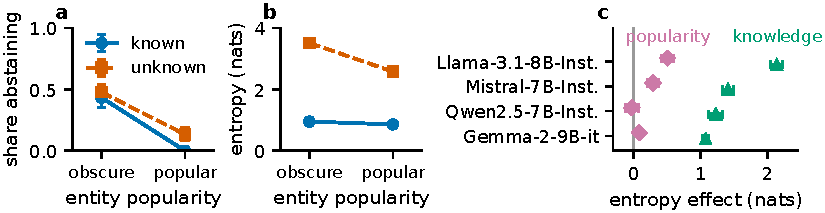
\includegraphics[width=\textwidth]{fig_dissociation.pdf}
\caption{\textbf{In Llama, saying \idk{} tracks popularity, while answer uncertainty follows knowledge.} (a) Llama-3.1-8B-Instruct: share of its free replies (chat template alone, three per question) that both LLM judges label \idk{} ($n=\hmLlamaItems$ questions; obscure known $n=\gsObsKnownTotal$). (b) Its entropy over the first answer token when the reply is forced to begin ``The answer is'' ($n=\faLlamaN$). (c) Popularity and knowledge effects on that entropy in four instruct models. Means with 95\% bootstrap intervals over questions.}
\label{fig:dissociation}
\end{figure}

About obscure entities, Llama says \idk{} in \hmLlamaObsKnown{} \lkObsKnownAbsCI{} of replies to questions it knows, against \hmLlamaPopKnown{} about popular entities (\cref{fig:dissociation}a), while forced-answer entropy in these two cells is \lkObsKnownEnt{} \lkObsKnownEntCI{} and \lkPopKnownEnt{} \lkPopKnownEntCI{} nats (\cref{fig:dissociation}b). Over the whole design the popularity effect on abstention is \hmLlamaPopEff{} \hmLlamaPopEffCI{} and the knowledge effect \hmLlamaKnowEff{} \hmLlamaKnowEffCI. Their difference, \hmLlamaDiff{} \hmLlamaDiffCI, equals obscure-known minus popular-unknown abstention, so it rests on those two cells. It keeps its sign under five other measurements, from \hjLlamaDiff{} to \faLlamaRegexDiff{} (\cref{app:robust}); the primary measure was designed after the smallest of these was seen. Answer entropy shows the reverse: it rises by \entLlamaKnow{} nats when Llama lacks the fact and by \entLlamaPop{} when the entity is obscure.

\emph{Labels.} Relabelling knowledge with a paraphrased question and prefix (fixed in advance) agrees with the original labels at $\kappa=\lcKappa$. Of the \gsObsKnownTotal{} obscure known facts, \eoObsKnownN{} stay known and abstain at \eoObsKnown; the difference is \eoDiff{} \eoDiffCI{} (\lcCons{} \lcConsCI{} where both labellings agree), and entropy still follows knowledge (knowledge minus popularity \eoEntKmP{} \eoEntKmPCI). Popular entities may have valid answers outside PopQA's aliases, so Llama-3.3-70B regraded forced answers by meaning (fixed in advance). It found \sePUKnown{} of the 100 popular unknown facts known and \sePUInter{} in between; with its labels the difference is \seDiff{} \seDiffCI.

\emph{Measurement.} With Llama-3.3-70B as a third judge and a majority rule, $\kappa=\tjLlamaKappa$ and the difference is \tjLlamaDiff{} \tjLlamaDiffCI. The \idk{} replies are refusals, not hedged answers: at most \lcDKAliasMax{} contain the gold alias in any cell, and counting only replies the 70B judge labels as declining without naming a candidate gives \sdDiff{} \sdDiffCI{} (fixed in advance).

\emph{Alternatives.} Llama describes the entity correctly in \ekObsKnown{} of its completions for obscure known facts and \ekPopKnown{} for popular known ones; as a covariate, this LLM-graded recognition measure shrinks the popularity effect by \ekShrink{} (fixed in advance). Ambiguity runs the wrong way (post hoc): popular subjects share their name with more Wikidata entities (median \amPopKnownHom--\amPopUnkHom) than obscure known ones (\amObsKnownHom), the \amSingleN{} obscure known facts with a unique name abstain at \amSingle, and a namesake-count covariate leaves the popularity coefficient at \amObs{} \amObsCI. Name form matters more in matched pairs of known facts (gap \scPopKnownGap{} falling to \scPopKnownGapSurface{} \scPopKnownGapSurfaceCI{} at equal surface form) than over all questions (\cref{app:robust}). Neither model-side measure shows the obscure names to be unfamiliar to Llama: name surprisal is uncorrelated with page views (\cref{app:surprisal}) and recognition is higher for obscure known facts. The result has the shape the misfire idea predicts but does not establish its mechanism.

\emph{One prompt.} At the forced-answer position, the first token's lean towards hedge tokens follows popularity and knowledge equally (\loLlamaDiff{} \loLlamaDiffCI; \cref{app:families}). After seeing this we read the free prompt: there the log-odds of a first token ``I'' follow popularity (\eoFreeIPop{} against \eoFreeIKnow) while its entropy follows knowledge (\eoFreeEntKnow{} against \eoFreeEntPop{} nats).

\subsection{Shared answer uncertainty; abstention measurable in Llama, and in Gemma when permitted}
\label{sec:families}

Entropy follows knowledge in all four families (\cref{fig:dissociation}c), as the labelling partly guarantees. Under the free prompt, Qwen, Gemma and Mistral rarely say \idk{} and the judges disagree on them; with a third judge Gemma reaches $\kappa=\tjGemmaKappa$ but abstains in at most \tjGemmaObsUnk{} of replies in any cell, so its preference cannot be estimated. The pre-registered four-family test on the forced-answer hedge readout returned Qwen \ffQwenVerdict, Gemma \ffGemmaVerdict{} and Mistral \ffMistralVerdict, but that readout shows no preference in Llama either (\cref{app:families}). When the question ends ``If you do not know the answer, say that you do not know'' (fixed in advance), both models abstain often and three judges agree ($\kappa=\pmLlamaKappa$, \pmGemmaKappa). Popularity minus knowledge is then \pmLlamaDiff{} \pmLlamaDiffCI{} for Llama and \pmGemmaDiff{} \pmGemmaDiffCI{} for Gemma, which says \idk{} to \pmGemmaObsKnown{} of obscure known questions and \pmGemmaPopKnown{} of popular known ones. Agreement between models on the forced-answer readout beyond shared labels met a post hoc rule for one of three pairs (\cref{app:crossmodel}).

\subsection{Mechanistic tests do not isolate a familiarity cause}
\label{sec:mech}

\begin{figure}[t]
\centering
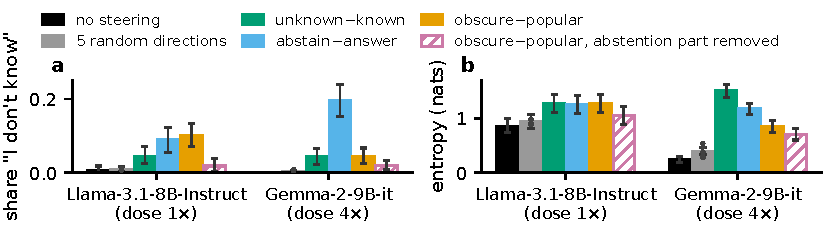
\includegraphics[width=\textwidth]{fig_steering.pdf}
\caption{\textbf{In Llama, steering along the obscure-minus-popular direction adds little abstention beyond its overlap with an abstention direction.} (a) Share of free replies both judges label \idk{} on 150 held-out popular questions each model knows; dots: random directions; hatched: obscure-minus-popular with its abstain-minus-answer component projected out. Gemma's two judges agree below the bar; three-judge rates in \cref{app:steer}. (b) First-token entropy under the forced-answer prompt. Error bars: 95\% bootstrap over questions.}
\label{fig:steering}
\end{figure}

\paragraph{Steering.} As work steering refusal along recognition directions does \citep{ferrando2025iknow,brzezinka2026familiarity}, we fitted obscure-minus-popular, unknown-minus-known and abstain-minus-answer directions on half of the questions \citep{arditi2024refusal,rimsky2024caa}, added each at a multiple (the dose) of the obscure-minus-popular direction's norm, chose the dose on a second set and scored a third (\cref{app:steer}). The obscure-minus-popular direction raised Llama's abstention from \svLlamaNone{} to \svLlamaFam, \svLlamaDOne{} \svLlamaDOneCI{} over random directions and short of the pre-set bar of $+0.10$ (\svLlamaMajDOne{} with three judges), and Gemma's from \svGemmaNone{} to \svGemmaFam{} at \svGemmaDose$\times$ the norm (\cref{fig:steering}a). In Llama it is nearly parallel to the abstention direction (cosine \svLlamaCos), partly by construction, since abstaining questions are mostly obscure. With that component removed it adds \svLlamaDTwo{} \svLlamaDTwoCI{} (Gemma \svGemmaDTwo{} \svGemmaDTwoCI). An abstention direction fitted on obscure questions alone (fixed in advance) still has cosine \wlLlamaCos, and removing it leaves \wlLlamaDTwo{} \wlLlamaDTwoCI{} (three judges). It beats unknown-minus-known on abstention (\svLlamaDThree{} \svLlamaDThreeCI), as the cells' rates predict, while in Gemma unknown-minus-known raises entropy \svGemmaDFour{} \svGemmaDFourCI{} nats more (\cref{fig:steering}b). Steering thus moves a generic abstention signal \citep[cf.][]{che2026steering}.

\paragraph{Lens.} Does a popularity-sensitive hedge signal exist before instruction tuning? With prefitted Jacobian lenses \citep{gurnee2026workspace} we read hedge tokens against answer-opening tokens at the forced-answer position in Llama-3.1-8B, Gemma-2-9B, Gemma-2-2B and OLMo-3-7B \citep{olmo3}. In the mid-depth window fixed in advance, popularity raises the hedge-token term in all four, but knowledge raises it at least as much; on the full readout, which the criterion also required, popularity exceeds knowledge in three of four because the answer-token term differs too (\cref{fig:lens}). Instruct partners lean further towards knowledge on the same readout (\cref{app:lens}), so the lens at this position does not show where Llama-Instruct's preference arises.

\section{Limitations and conclusion}

Abstention is judged by LLMs not validated against human labels. The design compares only the extreme page-view deciles, keeps only facts answered correctly at least nine times in ten or never, and caps cells at 100 questions; models have 2--9B parameters and questions name a single entity. Hedging driven by ambiguity that the judges do not label as clarification is not excluded. In this extreme-contrast design, Llama's answer uncertainty follows knowledge while its abstention tracks popularity more, so in Llama answer uncertainty alone predicts abstention poorly. Across families answer uncertainty agrees, partly by construction; abstention could be compared in two, and when permitted both track popularity more than knowledge.

\bibliographystyle{plainnat}
\bibliography{references}

\appendix

\section{Robustness of the Llama abstention result}
\label{app:robust}

\begin{table}[h]
\centering
\caption{Popularity effect minus knowledge effect on Llama's abstention under each measurement and labelling. Positive values mean abstention follows popularity more than knowledge. ``Corrected'': regex rates on 24-token replies corrected for the recall and precision of one LLM judge (Qwen2.5-32B-Instruct), measured on a subset labelled by that judge, not by people. $n$: questions.}
\small\begin{tabular}{p{5.3cm}p{2.5cm}rl}
\toprule
Measurement & Replies & $n$ & Popularity $-$ knowledge \\
\midrule
Regex detector & 20, 24 tokens & \faLlamaN & \faLlamaRegexDiff{} \faLlamaRegexDiffCI \\
One LLM judge, corrected & same 24-token & & \hjLlamaDiff{} \hjLlamaDiffCI \\
Two judges, both DONT\_KNOW (primary) & 3, 96 tokens & \hmLlamaItems & \hmLlamaDiff{} \hmLlamaDiffCI \\
Two judges, DONT\_KNOW or CLARIFY & same & \hmLlamaItems & \hmLlamaSecDiff{} \hmLlamaSecDiffCI \\
Regex detector & same & \hmLlamaItems & \hmLlamaRegexDiff{} \hmLlamaRegexDiffCI \\
Three judges, majority & same & \hmLlamaItems & \tjLlamaDiff{} \tjLlamaDiffCI \\
70B judge, declines naming no candidate & same & \hmLlamaItems & \sdDiff{} \sdDiffCI \\
Two judges, knowledge relabelled (paraphrase) & same & \lcBothN & \eoDiff{} \eoDiffCI \\
\quad both labellings agree (post hoc) & same & & \lcCons{} \lcConsCI \\
Two judges, unknown facts regraded by meaning & same & & \seDiff{} \seDiffCI \\
Two judges, popular unknown with alias in a reply dropped (post hoc) & same & & \lcAliasDrop{} \lcAliasDropCI \\
Two judges, guessable answers removed (post hoc) & same & & \gsDiff{} \gsDiffCI \\
Two judges, entity recognition as covariate$^{*}$ & same & \hmLlamaItems & \ekObs{} \ekObsCI \\
Two judges, namesake count as covariate$^{*}$ (post hoc) & same & & \amObs{} \amObsCI \\
\bottomrule
\end{tabular}

\smallskip\footnotesize $^{*}$Coefficient of the obscure arm in a linear probability model with relation fixed effects, not a difference of effects.
\end{table}

\emph{Design counts.} Llama's pool has \lkObsPoolKnown{} known, \lkObsPoolMaybe{} intermediate and \lkObsPoolUnk{} unknown obscure facts, and \lkPopPoolKnown{}, \lkPopPoolMaybe{} and \lkPopPoolUnk{} popular ones; the two-judge sample is a stratified random sample of 100 questions per cell (seed 0), or all of a smaller cell. Intervals for differences of cell means use 10,000 within-cell bootstraps (seed 0); linear probability models use 2,000 bootstraps over questions.

\emph{Measurements.} The single corrected judge gives the smallest difference. Its 24-token replies are often cut off before the model commits; why it and the regex disagree on the same replies is not established. The two-judge measurement with 96 tokens was designed for that reason after the \hjLlamaDiff{} was seen and made primary before it ran. Regex recall on the 96-token replies, against the two-judge labels, is \hmLlamaRegexRecall. Each judge's agreement with the three-judge majority: Qwen \lkMajQwen, Gemma \lkMajGemma, Llama-3.3-70B \lkMajLlama.

\emph{Independent labels} (criterion fixed in advance). Knowledge was relabelled with one paraphrased question per relation, the assistant prefix ``Answer:'' and fresh samples, under the same rule. Of the \lcBothN{} questions labelled under both prompts, \lcKK{} are known under both, \lcUU{} unknown under both, \lcKU{} known only originally and \lcUK{} only under the paraphrase (agreement \lcAgree, $\kappa=\lcKappa$); most other changes move popular known facts to the dropped band. Where both labellings agree, cells have \lcConsN{} questions (obscure unknown, obscure known, popular unknown, popular known). Under the new labels, the popularity effect on abstention is \eoPop{} \eoPopCI{} and the knowledge effect \eoKnow{} \eoKnowCI.

\emph{Regraded unknown facts} (criterion fixed in advance). Llama-3.3-70B graded each of a fresh greedy and ten sampled forced answers for every unknown fact as naming the gold entity or not. Of the 100 popular unknown facts in the sample, \sePUStay{} stay unknown, \sePUKnown{} become known and \sePUInter{} intermediate (dropped); of the 100 obscure unknown facts, \seOUStay{}, \seOUKnown{} and \seOUInter. Dropping instead every popular unknown question with a gold alias in any free reply (\lcPUAlias{} of them) gives \lcAliasDrop{} \lcAliasDropCI.

\emph{Strict declines} (criterion fixed in advance). The 70B judge labelled each reply as declining without naming a candidate, hedging with a candidate, answering, or asking which entity is meant. Declines occur in \sdObsKnown{} of obscure known replies and \sdPopKnown{} of popular known ones; among replies both judges call DONT\_KNOW, at most \sdHedgedMax{} per cell are hedged answers.

\emph{Entity recognition} (criterion fixed in advance). Llama completed ``\{subject\} is'' after the question ``What is \{subject\}?'' (greedy and five samples), and Llama-3.3-70B graded each completion against the subject's English Wikidata description; recognition is the share of completions graded correct. Its correlation with log page views over all graded questions is $\rho=\ekRho$. In the linear probability model its coefficient is \ekCoef{} \ekCoefCI{} per standard deviation, and it shrinks the popularity coefficient by \ekShrink{} on the two-judge measure and \ekShrinkRegex{} on the regex measure.

\emph{Guessable answers} (post hoc). An answer counts as guessable if a gold alias of at least three characters appears in the subject's name, or if it is its relation's most common answer and covers at least 20\% of the relation's pool. Among unknown facts alone the popularity gap in abstention is \hmLlamaPopUnkOnly{} \hmLlamaPopUnkOnlyCI. On the regex measure over the \gsRegexN{} non-guessable questions the difference is \gsRegexDiff{} \gsRegexDiffCI.

\emph{Namesakes} (post hoc). For each subject we counted Wikidata entities with the same English label; medians are \amObsKnownHom{} (obscure known), \amObsUnkHom{} (obscure unknown), \amPopKnownHom{} (popular known) and \amPopUnkHom{} (popular unknown). The covariate is the standardised log count.

\emph{Free replies} (post hoc). In the obscure known cell, \rcObsKnownCorrect{} of free replies contain a gold alias, and \rcObsKnownNonAbsCorrect{} of the replies that do not abstain; for \rcBothN{} of \rcBothOf{} questions, one free reply gives the correct answer and another says \idk. A linear probability model of abstention gives popularity \rcPopEnt{} \rcPopEntCI, knowledge \rcKnowEnt{} \rcKnowEntCI{} and \rcEntCoef{} per standard deviation of forced-answer entropy.

\emph{Name spelling} (post hoc). Over the \faLlamaN{} labelled questions, the popularity coefficient on the regex measure moves from \scPoolPop{} to \scPoolPopSurface{} logits per standard deviation after adding the name's word frequency, token count and token rarity. The matched pairs compare only known facts, one popular with one obscure fact of similar surface form, which is why they lose more of the gap.

\section{Abstention and the forced-answer hedge readout in all four families}
\label{app:families}

\begin{table}[h]
\centering
\caption{Judge agreement and abstention. Top: judge agreement and regex recall. Middle: abstention in the obscure, unknown cell. Bottom: three-judge abstention contrast, then effects on first-token hedge-versus-answer log-odds at the forced-answer position.}
\small\setlength{\tabcolsep}{3.5pt}\begin{tabular}{lcccc}
\toprule
& Llama & Qwen & Gemma & Mistral \\
\midrule
Two judges, $\kappa$ (bar \kappaBar) & \hmLlamaKappa & \hmQwenKappa & \hmGemmaKappa & \hmMistralKappa \\
Three judges, Fleiss $\kappa$ (bar \kappaBar) & \tjLlamaKappa & \tjQwenKappa & \tjGemmaKappa & \tjMistralKappa \\
Regex recall against two judges & \hmLlamaRegexRecall & \hmQwenRegexRecall & \hmGemmaRegexRecall & \hmMistralRegexRecall \\
\midrule
Both judges DONT\_KNOW & \hmLlamaObsUnk & \hmQwenObsUnk & \hmGemmaObsUnk & \hmMistralObsUnk \\
Both judges DONT\_KNOW or CLARIFY & \hmLlamaSecObsUnk & \hmQwenSecObsUnk & \hmGemmaSecObsUnk & \hmMistralSecObsUnk \\
Three judges, majority & \tjLlamaObsUnk & \tjQwenObsUnk & \tjGemmaObsUnk & \tjMistralObsUnk \\
Regex detector & \hmLlamaRegexObsUnk & \hmQwenRegexObsUnk & \hmGemmaRegexObsUnk & \hmMistralRegexObsUnk \\
\midrule
Three judges: popularity $-$ knowledge & \tjLlamaDiff & -- & \tjGemmaDiff & -- \\
Hedge log-odds: popularity & \loLlamaPop & \loQwenPop & \loGemmaPop & \loMistralPop \\
Hedge log-odds: knowledge & \loLlamaKnow & \loQwenKnow & \loGemmaKnow & \loMistralKnow \\
Hedge log-odds: popularity $-$ knowledge & \loLlamaDiff & \loQwenDiff & \loGemmaDiff & \loMistralDiff \\
Four-family verdict (pre-registered) & reference & \ffQwenVerdict & \ffGemmaVerdict & \ffMistralVerdict \\
\bottomrule
\end{tabular}
\end{table}

Intervals for the popularity-minus-knowledge rows: three judges, Llama \tjLlamaDiffCI, Gemma \tjGemmaDiffCI; hedge log-odds, Llama \loLlamaDiffCI, Qwen \loQwenDiffCI, Gemma \loGemmaDiffCI, Mistral \loMistralDiffCI. The two judges that agree best are Qwen2.5-32B and Llama-3.3-70B ($\kappa=\tjLlamaQwenLlamaK$ on Llama).

\emph{Permissive prompt} (criterion fixed in advance). The user message was the question followed by ``If you do not know the answer, say that you do not know.'', on each model's existing two-judge question set, with three replies scored by the three judges and a majority rule. Cell rates (obscure unknown, obscure known, popular unknown, popular known): Llama \pmLlamaObsUnk, \pmLlamaObsKnown, \pmLlamaPopUnk, \pmLlamaPopKnown; Gemma \pmGemmaObsUnk, \pmGemmaObsKnown, \pmGemmaPopUnk, \pmGemmaPopKnown. The criterion let Gemma's verdict replace ``cannot be estimated'' only if its obscure unknown rate reached 0.25.

\section{Steering details}
\label{app:steer}

Criterion fixed in advance (\cref{app:timing}). Directions were fitted on a random half of each model's questions at layer round$(0.55\times(L-1))$, the last position of the free prompt: obscure minus popular and unknown minus known (differences of cell means, each averaged over the other factor), and abstain minus answer (questions whose stored free-generation regex abstention rate is at least 0.5 minus those with rate 0). Their natural norms are \svLlamaNormFam, \svLlamaNormKnow{} and \svLlamaNormAbst{} in Llama and \svGemmaNormFam, \svGemmaNormKnow{} and \svGemmaNormAbst{} in Gemma. The obscure-minus-popular direction with its abstention component projected out was rescaled to the original norm. Each direction was added at a dose $k\in\{0.5,1,2,4,8\}$ times the obscure-minus-popular direction's natural norm, at the last prompt position and every generated position. $k$ was chosen on 150 popular known questions as the smallest value at which that direction beat five random directions by 0.10 in regex abstention, a rule separate from the confirmatory bar (\svLlamaDose$\times$ for Llama, \svGemmaDose$\times$ for Gemma, whose obscure-minus-popular regex rate was \svGemmaSelOne{} at 1$\times$ and \svGemmaSelTwo{} at 2$\times$). All conditions were scored on 150 further popular known questions, \lkSteerOverlap{} of which are also in the two-judge sample.

\begin{table}[h]
\centering
\caption{Share of steered replies both judges label \idk{} (regex detector in parentheses), 150 evaluation questions, 3 replies each.}
\scriptsize\setlength{\tabcolsep}{2.5pt}\begin{tabular}{lcccccc}
\toprule
& None & Random & Unk.$-$known & Abstain$-$answer & Obscure$-$popular & \dots{} abstention removed \\
\midrule
Llama & \svLlamaNone{} (\svLlamaNoneRegex) & \svLlamaRand & \svLlamaKnow{} (\svLlamaKnowRegex) & \svLlamaAbst{} (\svLlamaAbstRegex) & \svLlamaFam{} (\svLlamaFamRegex) & \svLlamaPerp{} (\svLlamaPerpRegex) \\
Gemma & \svGemmaNone{} (\svGemmaNoneRegex) & \svGemmaRand & \svGemmaKnow{} (\svGemmaKnowRegex) & \svGemmaAbst{} (\svGemmaAbstRegex) & \svGemmaFam{} (\svGemmaFamRegex) & \svGemmaPerp{} (\svGemmaPerpRegex) \\
\bottomrule
\end{tabular}
\end{table}

Primary scorer (both judges), obscure-minus-popular minus random: Llama \svLlamaDOne{} \svLlamaDOneCI, Gemma \svGemmaDOne{} \svGemmaDOneCI; with abstention removed: \svLlamaDTwo{} \svLlamaDTwoCI{} and \svGemmaDTwo{} \svGemmaDTwoCI; obscure-minus-popular minus unknown-minus-known: \svLlamaDThree{} \svLlamaDThreeCI{} and \svGemmaDThree{} \svGemmaDThreeCI. Secondary scorer (a majority of three judges, added by amendment before judging): obscure-minus-popular minus random \svLlamaMajDOne{} \svLlamaMajDOneCI{} and \svGemmaMajDOne{} \svGemmaMajDOneCI; with abstention removed \svLlamaMajDTwo{} \svLlamaMajDTwoCI{} and \svGemmaMajDTwo{} \svGemmaMajDTwoCI. For Gemma the secondary scorer is the defensible one, since its two judges agree below the bar. The regex detector counts far more abstentions than the judges for steered replies, so an earlier, regex-scored version of this experiment with the dose chosen on the evaluation questions (Llama \stLlamaNone{} to \stLlamaFam) overstated the effect. The cosine between the obscure-minus-popular and abstention directions is \svLlamaCos{} in Llama and \svGemmaCos{} in Gemma. No condition produced degenerate text.
\emph{Within-level abstention direction} (criterion fixed in advance). To remove the built-in overlap, the abstain-minus-answer direction was refitted on obscure questions only (\wlLlamaHi{} abstaining against \wlLlamaLo{} answering in Llama, \wlGemmaHi{} against \wlGemmaLo{} in Gemma), with the same splits, layer and dose, and scored by a majority of three judges. Its cosine with obscure-minus-popular is \wlLlamaCos{} in Llama and \wlGemmaCos{} in Gemma. Rates for no steering, the random mean, obscure-minus-popular, the within-level abstention direction and obscure-minus-popular with that direction removed: Llama \wlLlamaNone, \wlLlamaRand, \wlLlamaFam, \wlLlamaAbst, \wlLlamaPerp; Gemma \wlGemmaNone, \wlGemmaRand, \wlGemmaFam, \wlGemmaAbst, \wlGemmaPerp. Over random directions, obscure-minus-popular adds \wlLlamaDOne{} \wlLlamaDOneCI{} and \wlGemmaDOne{} \wlGemmaDOneCI, and with the within-level component removed \wlLlamaDTwo{} \wlLlamaDTwoCI{} and \wlGemmaDTwo{} \wlGemmaDTwoCI; Llama's pre-registered verdict is that the effect is carried by abstention. A first run launched with the two models' doses swapped produced degenerate Llama text and was discarded before analysis.

\section{Lens: window effects, the instruct models and onsets}
\label{app:lens}

Criterion fixed in advance. Hedge term: log-sum-exp of the lens log-probabilities of the hedge tokens `` not'', `` I'', `` unknown'', `` unclear'' and `` no''; the full readout subtracts the same quantity for the answer-opening tokens `` a'', `` the'', `` that'', `` in'', `` Yes'' and `` yes''. Window: relative depth $\ell/(L-1)\in[1/3,2/3]$. Intervals: 2,000 within-cell bootstraps. Each model was labelled known or unknown on its own prompt with the same sampling rule.

\begin{figure}[h]
\centering
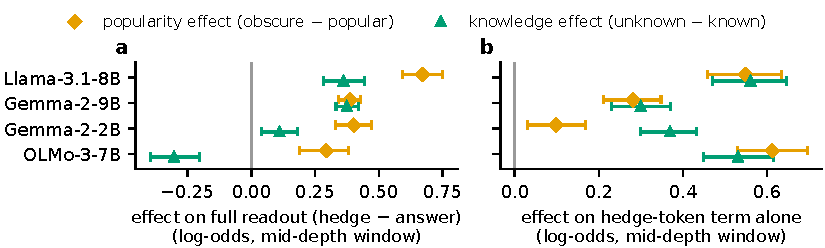
\includegraphics[width=\textwidth]{fig_lens_base.pdf}
\caption{\textbf{In base models, the decoded hedge readout responds to popularity, and at least as much to knowledge.} Jacobian-lens readout at the last position of ``Question: \ldots{} Answer: The answer is'', averaged over the pre-set mid-depth window: (a) log-odds of five hedge tokens (e.g.\ `` not'', `` unknown'') against six answer-opening tokens (e.g.\ `` the'', `` a''); (b) the hedge-token term alone. Points: popularity and knowledge effects with 95\% bootstrap intervals. Lenses are fitted per model, so magnitudes are not comparable across models.}
\label{fig:lens}
\end{figure}

\begin{table}[h]
\centering
\caption{Mid-depth window effects in base models, with 95\% intervals.}
\scriptsize\setlength{\tabcolsep}{3pt}\begin{tabular}{lcccc}
\toprule
& \multicolumn{2}{c}{Full readout} & \multicolumn{2}{c}{Hedge term alone} \\
\cmidrule(lr){2-3}\cmidrule(lr){4-5}
Model & Popularity & Knowledge & Popularity & Knowledge \\
\midrule
\lwRows
\bottomrule
\end{tabular}
\end{table}

\emph{Instruct partners} (criterion fixed in advance). The same readout, window and labelling rule were applied to Llama-3.1-8B-Instruct, Gemma-2-9B-it and Gemma-2-2B-it with their own prefitted lenses and chat-template forced-answer prompts. The criterion allowed the claim that instruction tuning increases the popularity preference only if, for a pair, the instruct difference exceeded the base difference with non-overlapping intervals; this held for no pair.

\begin{table}[h]
\centering
\caption{Popularity minus knowledge in the mid-depth window, base and instruct, with 95\% intervals. Lenses differ between the two models of a pair, so compare signs, not magnitudes.}
\scriptsize\setlength{\tabcolsep}{3pt}\begin{tabular}{lcccc}
\toprule
& \multicolumn{2}{c}{Full readout} & \multicolumn{2}{c}{Hedge term alone} \\
\cmidrule(lr){2-3}\cmidrule(lr){4-5}
Pair & Base & Instruct & Base & Instruct \\
\midrule
\itRows
\bottomrule
\end{tabular}
\end{table}

\emph{Onsets.} The onset of an effect curve is the first layer where it reaches half its positive maximum over layers and its 95\% interval excludes zero. A model supports the prediction that familiarity acts at a shallower depth than knowledge, our layer-depth analogue of a timing account of feelings of knowing \citep{koriat2001cascade}, if the knowledge onset follows the popularity onset with an interval above zero, and contradicts it if the interval lies below zero. The prediction was not supported (mixed): \jlSupports{} supporting, \jlContradicts{} contradicting and \jlUndecided{} undecided of the eight base and instruct models.

\begin{table}[h]
\centering
\caption{Lens onsets (layer index) of the popularity (F) and knowledge (K) effects, their difference $D=K-F$ with its 95\% interval, the outcome, and the mid-depth popularity effect on the full readout. Instruct rows use the instruct models' own lenses.}
\footnotesize\begin{tabular}{lcccccc}
\toprule
Model & Layers & F onset & K onset & $D$ & Outcome & Mid popularity \\
\midrule
\jlOnsetRows
\bottomrule
\end{tabular}
\end{table}

\section{Cross-model agreement (exploratory)}
\label{app:crossmodel}

Spearman correlations across questions between Llama's and each other model's forced-answer hedge log-odds and first-token entropies, on questions where both models have the same knowledge label and where they differ (95\% bootstrap intervals). The plan, including the rule that hedge agreement and the hedge-minus-entropy gap both have 95\% intervals excluding zero, was written before this run, but the point estimates had been seen, so the analysis is post hoc.

\begin{table}[h]
\centering
\footnotesize\begin{tabular}{lccc}
\toprule
& Llama--Qwen & Llama--Gemma & Llama--Mistral \\
\midrule
Questions, knowledge differs & \cmQwenDiffN & \cmGemmaDiffN & \cmMistralDiffN \\
Hedge log-odds agreement & \cmQwenDiffHedge{} \cmQwenDiffHedgeCI & \cmGemmaDiffHedge{} \cmGemmaDiffHedgeCI & \cmMistralDiffHedge{} \cmMistralDiffHedgeCI \\
Entropy agreement & \cmQwenDiffEnt{} \cmQwenDiffEntCI & \cmGemmaDiffEnt{} \cmGemmaDiffEntCI & \cmMistralDiffEnt{} \cmMistralDiffEntCI \\
Gap (hedge $-$ entropy) & \cmQwenDelta{} \cmQwenDeltaCI & \cmGemmaDelta{} \cmGemmaDeltaCI & \cmMistralDelta{} \cmMistralDeltaCI \\
Rule & \cmQwenRule & \cmGemmaRule & \cmMistralRule \\
\midrule
Questions, same knowledge & \cmQwenSameN & \cmGemmaSameN & \cmMistralSameN \\
Hedge log-odds agreement & \cmQwenSameHedge & \cmGemmaSameHedge & \cmMistralSameHedge \\
Entropy agreement & \cmQwenSameEnt & \cmGemmaSameEnt & \cmMistralSameEnt \\
\bottomrule
\end{tabular}
\end{table}

\section{A model-side familiarity measure (negative result)}
\label{app:surprisal}

Criterion fixed in advance. We computed the mean per-token surprisal of each subject name under the base Llama-3.1-8B in the context ``Here is a name:''. It is uncorrelated with log page views (Spearman \esRho). With knowledge and name length held fixed, its coefficient per standard deviation is \esJudge{} \esJudgeCI{} on two-judge abstention and \esRegex{} \esRegexCI{} on the regex measure; adding the popularity arm moves the regex coefficient to \esRegexPop{} \esRegexPopCI, although surprisal hardly correlates with the arm (point-biserial \esArmR; \esArmPartial{} given relation and knowledge), which we have not resolved. Surprisal therefore does not stand in for popularity. Short names made of common words (``New York'' as a book title) are a likely reason.

\section{Timing, neurons and the circuit}
\label{app:circuit}

On matched pairs of obscure and popular questions in Llama, the lens-decoded abstention readout reaches half its final size at layer \ltHedgeHalf, while the entropy gap does so at layer \ltEntHalf, \ltLead{} layers later; this compares two readouts of one contrast, not the onsets in \cref{app:lens}. Neurons selected for their correlation with output entropy in Llama and Qwen behaved as word-frequency and temperature neurons \citep{stolfo2024confidence,gurnee2024universal}. A set of 20 attention heads and 100 MLP neurons found by activation patching \citep{wang2023ioi,syed2023attribution} reproduces \ciRecovery{} \ciRecoveryCI{} of the first-token abstention log-odds difference when patched from popular into obscure questions and \ciRecoveryUC{} \ciRecoveryUCCI{} from obscure into popular ones; in generation, removing its state removes abstention in \ciRemoveFlip{} of cases but injecting it produces abstention in only \ciInjectFlip, short of a behavioural bar fixed in advance. Shared uncertainty circuits \citep{teplica2025sciurus}, a commit-or-abstain circuit across ten models \citep{nguyen2026commit} and a similar asymmetry between releasing and restoring refusal \citep{liu2026broken} have been reported before.

\section{Analysis timing}
\label{app:timing}

Each confirmatory analysis had a criterion note written before its run, stating the measurement, the test and the wording each outcome would license; the SHA-256 prefix of each note was recorded before the run, and the notes are in the supplementary material. Four-family design: \hashQwenFactorial, \hashGemmaMistralFactorial; one corrected judge: \hashHedgeJudge; two-judge measurement: \hashHedgeMeasure; lens study: \hashLens; circuit behaviour: \hashCircuit; independent labels: \hashEOne; name surprisal: \hashETwo; lens split: \hashEThree; steering with held-out dose: \hashEFour{} (amendment adding the third judge as a secondary scorer: \hashEFourA; its internal date is a day later than its recorded hash time, a dating error in the note itself); third judge: \hashEFive; entity recognition: \hashESix; regraded labels and strict declines: \hashESeven; steering with a within-level abstention direction: \hashEEight; permissive prompt: \hashENine; instruct lens: \hashETen. An earlier steering experiment (\hashSteering, \hashNoHedge) is superseded by the held-out design. The guessability, namesake, spelling, free-reply, entropy-control and label-agreement checks and the cross-model agreement were decided after seeing data and are post hoc.

\end{document}
